\documentclass[10pt, landscape, a4paper]{article}
\usepackage[margin=0.1in,  footskip=7pt, includefoot]{geometry}
\usepackage{multicol}
\usepackage{blindtext} % this can be removed later on
\usepackage{titlesec}
\usepackage{xcolor}
\usepackage{amsmath}
\usepackage{graphicx}
\usepackage{amssymb}
\usepackage{mathptmx}
\usepackage{paralist} 
\usepackage{wrapfig}
\usepackage{fancyhdr}  % Add this package for page numbers
\usepackage{tabularx}

\usepackage{ulem}  % For underlining


\graphicspath{{assets/}}


% Reduce spacing before and after sections
\titlespacing{\section}{0pt}{0.5\baselineskip}{0.5\baselineskip}
\setlength{\columnseprule}{1pt} % Add lines between columns

% Set indentation
\setlength{\parindent}{0pt}
\setlength{\parskip}{0cm}

\titlespacing{\section}{0pt}{0.5ex}{0ex}
\titlespacing{\subsection}{0pt}{0.5ex}{0ex}
%\linespread{0.9}

\newcommand*{\myfont}{\fontfamily{phv}\selectfont}


% Define custom colors
\definecolor{darkblue}{RGB}{0, 0, 139}  % Adjust RGB values as needed
\definecolor{darkgreen}{RGB}{0, 100, 0}  % Adjust RGB values as needed
\definecolor{definitionColor}{RGB}{150, 0, 150}
\definecolor{lightgray}{RGB}{200, 200, 200}

\newcommand{\greenbf}[1]{\textcolor{definitionColor}{\textbf{#1}}}
\newcommand{\bluebf}[1]{\textcolor{darkblue}{\textbf{#1}}}
\newcommand{\graytext}[1]{\textcolor{lightgray}{\footnotesize #1}}



\newcommand{\E}[0]{\mathbb{E}}
\newcommand{\N}[0]{\mathbb{N}}
\newcommand{\R}[0]{\mathbb{R}}

\newcommand{\sgn}[0]{\text{sgn}}

\newcommand{\argmin}[1]{\underset{#1}{\text{argmin}}}
\newcommand{\argmax}[1]{\underset{#1}{\text{argmax}}}



\titlespacing{\section}{0pt}{0.5ex}{0ex}
\titlespacing{\subsection}{0pt}{0.5ex}{0ex}
%\linespread{0.9}

% NEED TO ADD:
% SHADING
\pagestyle{fancy}
\fancyhf{}  % Clear existing headers and footers
\rfoot{\thepage}  % Page number at the bottom-right corner

\begin{document}


\begin{multicols}{4}

% Your content goes here

% \section{Introduction}
% \blindtext
% \section{Body}



\section{The Digital Image}
\greenbf{Problems:} Transmission interference, compression artifacts, spilling, scratches, sensor noise, bad contrast and resolution, motion blur \\
\greenbf{Pixel:} Discrete samples of an continuous image function.\\
\greenbf{Rolling Shutter} effect produced by sequential readout of pixels while a digital camera is moving. Result is pixels read at different times are sequentially misaligned, causing image-level distortions dependent on camera (or object) movement.
\subsection*{Charge Coupled Device \graytext{(CCD)}}
Has an array of photosites \graytext{(a bucket of electrical charge)} that charge proportional to the incident light intensity during exposure. ADC happens line by line. \\
\greenbf{Bloooming:} oversaturation of finite capacity photosites causes the vertical channels to "flood" \graytext{(bright vertical line)}\\
\greenbf{Bleeding/Smearing:} While shifting down, the pixels above get some photons on bright spot with electronic shutters.\\
\greenbf{Dark Current:} CCDs produce thermally generated charge they give non-zero output even in darkness \graytext{(fluctuates randomly)} due to spontaneous generation of electrons due to heat $\rightarrow$ cooling.\\ can be avoided by cooling, worse with age.
\subsection*{CMOS:}
Same sensor elements as CCD, but each sensor has its own amplifier $\rightarrow$ faster readout, less power consumption, cheaper, more noise.\\ more noise, lower sensitivity\\
\greenbf{vs CCD} cheaper, lower power, less sensitive, per pixel amplification random pixel access, no blooming, on chip integration
\subsection*{Sampling methods}
Cartesian \graytext{(grid)}, hexagonal, non-uniform\\
\greenbf{Quantization:} Real valued function will get digital values \graytext{(integers)}. A lossy process \graytext{(original cannot be reconstructed)}. Simple version: equally spaced $2^b = \#bits$ levels\\
\greenbf{Linear Interpolation}: \\
$p(t) = p_0 + (t - t_0)\frac{p_1 - p_0}{t_1 - t_0} \text{ with } t \in [t_0, t_1]$ \\

\greenbf{Bilinear Interpolation:}     \\
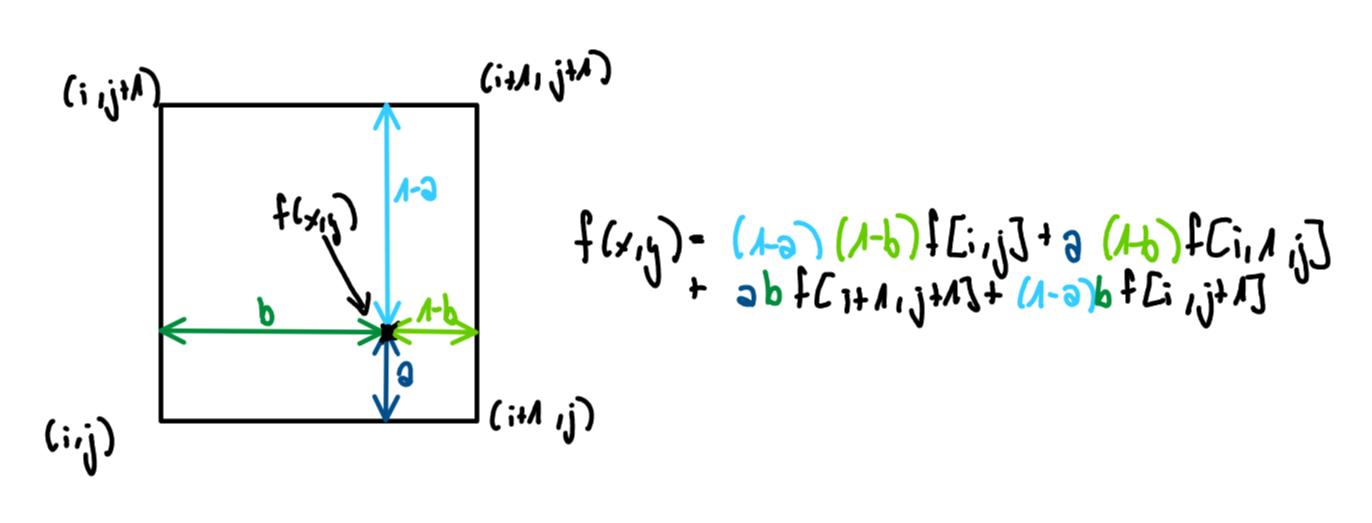
\includegraphics[width=\columnwidth]{jo/linear-interpolation.png} \\ 
\greenbf{Resolution:} Image resolution \graytext{(cropping)}, geometric resolution \graytext{(\#pixels per area)}, radiometric resolution \graytext{(\#bits per pixel, color)}\\
\greenbf{Image noise:} commonly modeled by additive Gaussian noise: $I(x, y) = f(x, y) + c$, poisson noise \graytext{(shot noise for low light, depends on signal \& aperture time)}, multiplicative noise: $I = f + f \cdot c$, quantization errors, salt-and-pepper noise. SNR or peak SNR is used as an index of image quality $c \sim N(0, \sigma^2)$, $p(c) = \frac{1}{\sigma \sqrt{2\pi}} \cdot \exp\left(-\frac{(c - \mu)^2}{2\sigma^2}\right)$, SNR: $S = \frac{F}{\sigma}$ where $F = \frac{1}{XY}\sum_{x = 1}^X \sum_{y = 1}^{Y} f(x, y)$.
\subsection*{Color cameras}
\greenbf{Prism} need 3 sensors and good alignment\\
\greenbf{Filter mosaic} coat $\square$ directly on sensor \\
\greenbf{Wheel} multiple filters in front of same sensor\\
\greenbf{New CMOS sensor} layers that absorb color at different depths $\rightarrow$ better quality
\section*{Image Segmentation}
\subsection*{Complete segmentation}
Finite set of non-overlapping regions that cover the whole image $I = \bigcup_{i = 1}^{n} R_i$ and $R_i \cap R_j = \emptyset$ $\forall i, j, i \neq j$\\
\greenbf{Thresholding:} simple segmentation by comparing greylevel with a threshold to decide if in or out.\\
\greenbf{Chromakeying:} when planning to segment, use special backgroundcolor. (Problems variations due to lighting, noise, ... mixed pixels (hard $\alpha$-mask does not work)) $I_\alpha = |I - g| > T$
\subsection*{Receiver Operating Characteristic (ROC) analysis:}
ROC curve characterizes performance of binary classifier Classification errors: False negative (FN), false positives (FP)\\
ROC curve plots TP fraction $\frac{TP}{TP + FN}$ vs FP fraction $\frac{FP}{FP + TN}$\\
\greenbf{Operating points:} choose point with gradient
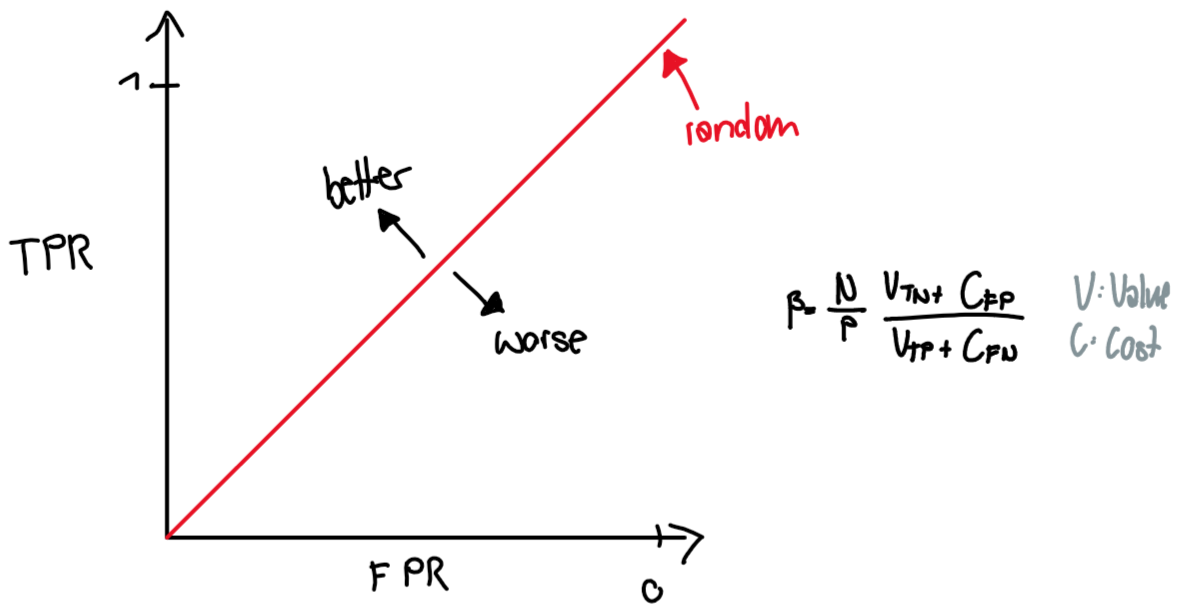
\includegraphics[width=0.4\columnwidth]{jo/roc.png} 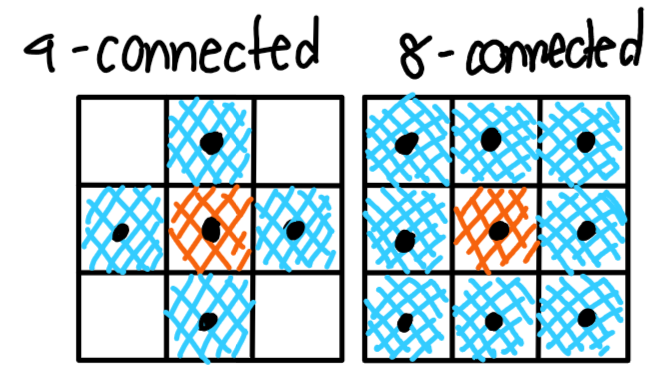
\includegraphics[width=0.4\columnwidth]{jo/connection.png}
\subsection*{Pixel connectivity}
\graytext{also regions if $x$-connected}\\
\greenbf{Connected component raster scanning:} scanning row by row, if foreground \& label if connected to other label, else give new label. (second pass to find equivalent labels)\\
\greenbf{Improve:} when region found, follow border, then carry on (contour-based method)
\subsection*{Region growing}
Start with seed point or region, add neighboring pixels that satisfy a criteria defining a region until we include no more pixels.\\
\greenbf{Seed region:} by hand or automatically by conservative Thresholding\\
\greenbf{Inclusion criteria:} greylevel thresholding, greylevel distribution model (include if ($I(x, y) - \mu^{2})^{2} < (n \sigma)^{2}$ and update $\mu$ and $\sigma$ after each iteration) color or texture information\\
\greenbf{Snakes:} active contour, a polygon and each point moves away from seed while criteria is met (can have smoothness constraint) Iteratively minimize enery function $E = E_{tension} + E_{stiffness} + E_{image}$
\subsection*{background subtraction}
simple: $I_\alpha = |I - I_{bg}| < T$ better: $I_\alpha = \sqrt{(I - I_{bg})^T \Sigma^{-1} (I - I_{bg})}$ where $\Sigma$ is the background pixel appearance covariance matrix, computed seperately for each pixel.
\subsection*{Morphological operators}
Logical transformations based on comparison of neighboring pixels\\
\greenbf{erode} delete FG pixels with 8-connected BG pixels\\
\greenbf{dilate} every BG pixels with 8-connected FG pixel make a FG pixel\\
\greenbf{Uses:} smooth regions, remove noise and artifacts.
\section{Image Filtering}
\greenbf{Local Filter:} A filter is local if it modifies pixels based on neighborhood.\\
Modify the pixels of an image based on some function of the local neighborhood of the pixels- If sum greater 1 get brighter, if smaller darker.\\
\greenbf{shift invariant:} Doing the same thing, applying the same function over all pixels (in the formula below if $K$ does not depend on $x, y$)\\
\greenbf{Linear Filtering}\\
$L$ is linear operation if $L[\alpha I_1 + \beta I_2] = \alpha [I_1] + \beta L[I_2]$\\
\greenbf{Linear:} linear combination of neighbors can be written as: \\
$\sum_{\begin{subarray}{c}
    (i, j) \in \underbrace{\mathbb{N}(x, y)}_{\text{neighborhood}}
\end{subarray}}
K(x, y, i, j) \underbrace{I}_{\text{Input}} (x + i, y + j)$

\greenbf{Filter at edges:} clip filter (black), wrap around, copy edge, reflect across edge, vary filter near edge
\subsection*{Correlation}
$I'(x, y) = \sum_{(i, j) \in \N(x, y)} K(i, j) I (x + i, y + j)$ \\
$I' = K \circ I \quad$ e.g. template matching: search for best match by minimizing mean squared error or maximizing area correlation. (remove mean (from filter, from image) to avoid bias)
\subsection*{Convolution}
$I' = K * I, I'(x, y) = \sum_{(i, j) \in \N(i, j)} K(i, j) I (x - i, y - j)$ if $K(i, j) = K (-i, -j) \implies \\
correlation = convolution \quad\\
convoution = correlation + \text{ filter rotated 180°}$\\
\greenbf{Continuous:} $(f * g)(t) \\
= \int_{-\infty}^{\infty} f(\tilde{t}) g(t - \tilde{t}) d\tilde{t}\\
= \int_{-\infty}^{\infty} f(t - \tilde{t}) g(\tilde{t}) dt$
\subsection*{Kernels}
\greenbf{separable:} if a kernel can be written as a product of two simpler filters $\rightarrow$ computationally faster (filter $P \times Q$, image $N \times M: (P + Q) * NM$ instead of $PQNM$)\\
Separable filters can be written as \( K(m,n) = f(m)g(n) \).
For a rectangular neighborhood with size \((2M+1) \times (2N+1), I'(m, n) = \fcolorbox{green}{white}{f * (\fcolorbox{red}{white}{g * I(N(m, n))})}\)\\
$
\fcolorbox{red}{white}{I''(m,n)} = \sum_{j=-N}^{N} g(j) I(m, n - j)
$
\\
$\fcolorbox{green}{white}{I'(m, n)} = \sum_{j=-N}^{N} f(i) I''(m - i, n)$\\
\greenbf{Box filter:} all same values normalized to sum = 1\\
\greenbf{Gaussian Kernel:} $K(x, y) = \frac{1}{2\pi \sigma^{2}} e^{-\frac{x^{2} + y^{2}}{2\sigma^{2}}}$ is separable, e.q. $\sigma = 1$\\
Gaussian Smoothing Kernel Top-5
\begin{compactitem}
\item Rotationally symmetric
\item has single lobe \graytext{Neighbor's influence decreases monotonically}
\item Still one lobe in frequency domain ,\graytext{No corruption from high frequencies}
\item Simple relationship to $\sigma$
\item Easy to implement efficiently
\end{compactitem}
\greenbf{High Pass Filter:}
high pass filter detects edges 
High Pass Filter Laplacian Operator \\
$
\begin{bmatrix}
   % \begin{smallmatrix}
        -1 & -1 & -1 \\
        -1 & 8 & -1 \\
        -1 & -1 & -1 \\
    %\end{smallmatrix}
\end{bmatrix} 
$$
\begin{bmatrix}
    %\begin{smallmatrix}
        0 & 1 & 0 \\
        1 & -4 & 1 \\
        0 & 1 & 0 \\
    %\end{smallmatrix}
\end{bmatrix} 
$
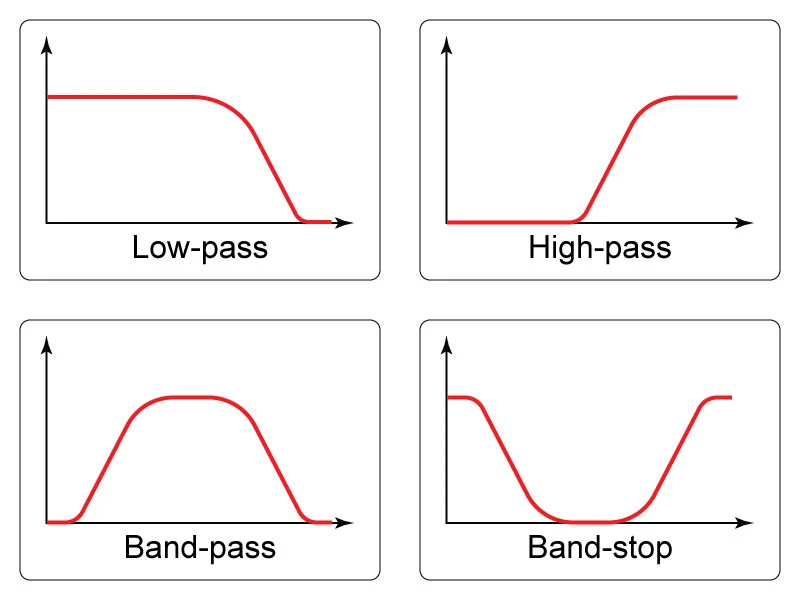
\includegraphics[width = 0.3 \columnwidth]{assets/jo/Types_of_Filters.png}

\greenbf{Low Pass Filter:}
blurs (detects "smooth" regions) Gaussian Filter is a low pass filter, proof: Convolution theorem: Fourier transform H of h is equal to $F \cdot G$
If $g$ is Gaussian, its Fourier Transform $G$ is also Gaussian.
Pointwise multiplication of $F$ with $G$ will keep the low frequencies of F unchanged, while the high frequencies will be multiplied by a low number, and therefore, they will be removed.  \\
\greenbf{Conversion:} Subtracting one from central element of low-pass filter gives a high-pass filter with inverted sign, because.\\
$(f - \delta) * a = f * a - \delta * a = f * a - a = - (a - (f * a))$ Normalize the low-pass kernel and then subtract one from central element. Normalize low-pass filter, then subtract the kernel from central element matrix. To get the high pass filter, you do not need to normalize.\\
\greenbf{Band pass filter:} 
\includegraphics*[width = 0.4cm]{jo/band-pass-filter.png}
do LPF and HPF with cutoffs $f_{LP} < f_{HP} \quad f = \text{ cut of frequencies, cannot coincide}$\\
Filter image with high-pass and low-pass filter to get band pass filter. \graytext{Only works when you have an overlap in frequencies. If no overlap: $I *_{convolution} (\delta - f_{LP - f_{HP}}) \rightarrow $ gap between is band filter.}\\
\greenbf{Band reject filter:} \includegraphics*[width = 0.4cm]{jo/band-reject-filter.png}
do LPF and HPF with cutoffs $f_{LP} > f_{HP}$\\
\greenbf{Image sharpening:} increases high frequency components to enhance edges: $I' = I + \alpha |K * I|$ $K:$ high-pass filter, $\alpha$: scalar $\in [0, 1]$
\section{Features}
\greenbf{Desirable properties:} shift, rotation, scale, brightness invariant
\subsection*{Edge Detection}
How to tell if there is an edge? Local maxima of the first derivative and the zero crossing of the second derivative.\\
\greenbf{Edge detection filters:}

\greenbf{Sobel:}\\
$K_x = \begin{bmatrix}
    \begin{smallmatrix}
        -1 & 0 & 1\\
        -2 & 0 & 2\\
        -1 & 0 & 1
    \end{smallmatrix}
\end{bmatrix}$,
$K_y = \begin{bmatrix}
    \begin{smallmatrix}
        -1 & -2 & -1\\
        0 & 0 & 0\\
        1 & 2 & 1
    \end{smallmatrix}
\end{bmatrix}$

\greenbf{Prewitt:}\\
$K_x = \begin{bmatrix}
    \begin{smallmatrix}
        -1 & 0 & 1\\
        -1 & 0 & 1\\
        -1 & 0 & 1
    \end{smallmatrix}
\end{bmatrix}$,
$K_y = \begin{bmatrix}
    \begin{smallmatrix}
        -1 & -1 & -1\\
        0 & 0 & 0\\
        1 & 1 & 1
    \end{smallmatrix}
\end{bmatrix}$

\greenbf{Roberts:}\\
$K_x = \begin{bmatrix}
    \begin{smallmatrix}
        1 & 0\\
        0 & -1
    \end{smallmatrix}
\end{bmatrix}$,
$K_y = \begin{bmatrix}
    \begin{smallmatrix}
        0 & 1\\
        -1 & 0
    \end{smallmatrix}
\end{bmatrix}$

\greenbf{Gradient Magnitude:}\\
$M(x, y) = \sqrt{(\frac{\partial f}{\partial x})^{2} + (\frac{\partial f}{\partial y})^{2}}$\\
\greenbf{Gradient Angle:} \\
$\alpha(x, y) = \tan^{-1}(\frac{\partial f}{\partial y} / \frac{\partial f}{\partial x})$
\subsection*{Laplacian operator}
detect discontinuities by considering second derivative
$\begin{bmatrix}
    \begin{smallmatrix}
        0 & 1 & 0\\
        1 & -4 & 1\\
        0 & 1 & 0
    \end{smallmatrix}
\end{bmatrix}
\quad \text{or} \quad
\begin{bmatrix}
    \begin{smallmatrix}
        1 & 1 & 1\\
        1 & -8 & 1\\
        1 & 1 & 1
    \end{smallmatrix}
\end{bmatrix}$
are discrete space approximations. Is isotropic\graytext{(rotationally invariant)}, zero crossings make edge locations. Sensitive to fine details and noise \graytext{($\rightarrow$ smoothing before applying)}.\\ blur image first \graytext{(LoG)}\\
\greenbf{Laplacian of Gaussian \graytext{(LoG)}:} convolve gaussian blurring and laplacian operator in LoG operator \graytext{(cheaper)} $LoG(x, y) = -\frac{1}{\pi \sigma^{4}} (1 - \frac{x^{2} + y^{2}}{2\sigma^{2}}) e^{-\frac{x^{2} + y^{2}}{2\sigma^{2}}}$
\subsection*{Canny Edge Detector: 5 Steps}
\begin{compactenum}
    \item smooth image with a Gaussian filter
    \item compute gradient magnitude and angle using Sobel/Prewitt/...
    \item apply non-maximum suppression to gradient magnitude image \graytext{(Quantize edge normal to one of four directions: horizontal, +45°, vertical, -45°. If $M(x, y))$ smaller than either of its neighbors in edge normal direction suppress, else keep}
    \item Double thresholding for intensity to detect strong and weak edge pixels
    \item Reject weak edge pixels not connected to strong edge pixels
\end{compactenum}
\subsection*{Hough Transform}
Fitting a straight line to a set of edge pixels\\
\includegraphics*[width = \columnwidth]{jo/slope.png}\\
\greenbf{Alternative parameterization:}\\
$x \cos(\theta) + y \sin(\theta) = \rho$ \\
$(x - a)^{2} + (y - a)^{2} = r^{2}$
\greenbf{For circles:} if r known: calculate circles with radius r around edge pixels $\rightarrow$ intersection (local maxima) of circles gives center.\\ Where lots of them meet is the center of a circle. else: use 3D hough transform with parameters $(x_0, y_0, r)$
Each point $(x_i, y_i)$ in the $xy$-plane gives a sinusoid in the $\theta \rho$ plane. Colinear points lying on the line give curves intersecting at the same point in the polar parameter plane. Local maxima give significant lines.
\subsection*{Corner Detection}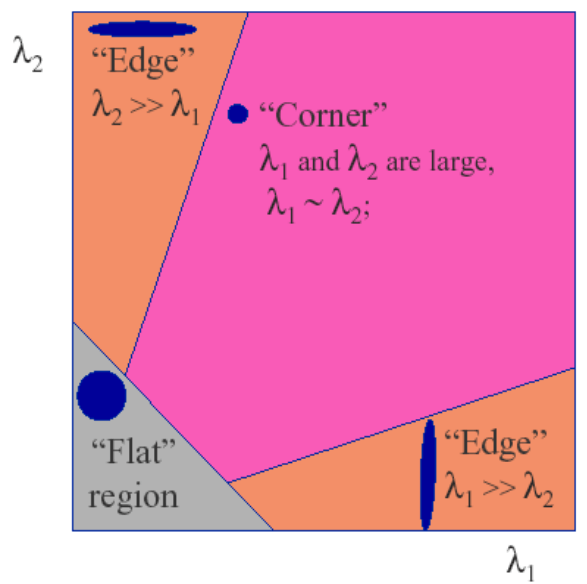
\includegraphics[width = 2cm]{jo/corner.png}\\
Edges are only well localized in one direction $\rightarrow$ detect corners.\\
Desirable properties: Acute localization, invariance against shift, rotation, scale, brightness change, robust against noise, high repeatability\\
\greenbf{Linear approximation for small $\Delta x \Delta y$:} (Taylor) $f(x + \Delta x, y + \Delta y) \approx f(x, y) + f_x(x, y) \Delta x + f_y(x, y)\Delta y$
\subsection*{Local displacement sensitivity \graytext{(Harris corners)}}
$S (\Delta x, \Delta y) = (\Delta x \Delta y) \left( \sum_{x, y \in \text{window}}
\begin{bmatrix}
    \begin{smallmatrix} 
        f_x^{2} & f_x f_y \\ 
        f_x f_y & f_y^{2} 
    \end{smallmatrix} 
\end{bmatrix}
\right)
\begin{bmatrix}
    \begin{smallmatrix} 
        \Delta x \\ 
        \Delta y
    \end{smallmatrix} 
\end{bmatrix}  \\
\approx \text{SSD}$.
Find points where $\min \Delta^T M \Delta$ is large for $||\Delta || = 1$ i. e. maximize the eigenvalues of $M$\\
\greenbf{Harris cornerness:} Measure of cornerness\\
$C(c, y) = \det(M) - k * trace(M)^{2} = \lambda_1\lambda_2 + k(\lambda_1 + \lambda_2)$ \\
\greenbf{Robustness of Harris corner detector:} Invariant to brightness offset, invariant to shift and rotation but not to scaling!
$\lambda_1 >> \lambda_2 \rightarrow$ edge, $\lambda_1$ and $ \lambda_2$ large $\rightarrow$ corner, else $\rightarrow$ flat region.\\
not scale invariant: \includegraphics*[width = 4cm]{jo/corner-edge.png}\\
\greenbf{Overcome issues:} look for strong DoG response or consider local maxima in position and scale space, Gaussian weighing.
\subsection*{Lowe's SIFT features}
Look for strong responses of difference of Gaussians \graytext{(DoG)} filter, only look at local maxima in both position and scale.\\
\greenbf{DoG:} $DoG(x, y) = \frac{1}{k}* e^{-\frac{x^{2} + y^{2}}{(k\sigma)^{2}}} - e^{-\frac{x^{2} + y^{2}}{\sigma^{2}}}$ e.g. $k = \sqrt{2}$\\
Orientation: create histogram of local gradient directions computed at selected scale, assign canonical orientation at peak of smoothed histogram. Get a SIFT descriptor \graytext{(threshold image gradients are sampled over $16\times 16$ array of locations in scale space)} and do matching with these. Invariant to scale, rotation, illumination and viewpoint.



\section{Fourier Transformation}
\greenbf{Aliasing:} Happens when undersampling e.g. taking every second pixel, else characteristic errors appear: typically small phenomena look bigger, fast phenomena look slower. (e.g. wagon wheels backwards in movies, checkerboards misrepresented)
\subsection*{Fourier Transform}
\greenbf{Convolution, Filtering:} The Fourier transform of the convolution of two functions is the product of their Fourier transform:\\
$F \cdot G = U(f ** g)$\\
\greenbf{Convolution, Sampling:} The Fourier transform of the product of two functions is the convolution of the Fourier transform.\\
$F ** G = U(f \cdot g)$\\
%$\sin(x) = \frac{e^{ix} - e^{-ix}}{2i}$\\
%$\cos(x) = \frac{e^{ix} + e^{-ix}}{2}$\\
Represent function on a new basis with basis elements $e^{i 2 \pi (ux + vy)} = \cos(2 \pi (ux + vy)) + i \sin(2 \pi (ux + vy))$\\
$F(f(x))(u) = \int_{-\infty}^{\infty} f(x) e^{-i 2 \pi ux} dx$, \\
\greenbf{Inverse Fourier:} $f(x) = \int_{\infty}^{\infty} F(u)e^{i2\pi ux} du$ Similar for 2D \\
\greenbf{2D:} $F(f(x,y))(u, v) = \int_{-\infty}^{\infty} \int_{-\infty}^{\infty} f(x, y) e^{-2\pi i (ux + vy)}dx dy$\\
\greenbf{For images:} transformed image $\rightarrow$ $F = U * f$ $\leftarrow$ vectorized image, U: Fourier matrix\\
\greenbf{For discrete:} \\$F(u, v) = \frac{1}{NM}\sum_{x=0}^{N-1} \sum_{y=0}^{M-1} f(x, y) e^{-2\pi i (\frac{ux}{N}, \frac{vy}{M})}$\\ % source: Processing Signals Slide 15
\greenbf{1D-periodic function:} $f(t) = \sum_{n = -\infty}^{\infty} c_n e^{\frac{i 2 \pi n t}{T}}$, $c_n = \frac{1}{T} \int_{-\frac{T}{2}}^{\frac{T}{2}} f(t) e^{\frac{-i 2 \pi n t}{T}} dt$
\subsection*{Properties of Fourier transform}
\greenbf{Linearity:} $F(ax(t) + by(t)) = aX(t) + bY(t)$\\
\greenbf{Time Shift:} $F(x(t \pm t_0)) = X(t) e^{\pm i 2 \pi f t_0}$\\
\greenbf{Frequency Shift:} $F(e^{i 2 \pi f_0 t} x(t)) = X(f - f_0)$\\
\greenbf{Scaling:} $F(x(at)) = \frac{1}{|a|}X\left(\frac{f}{a}\right)$\\
\greenbf{Convolution:} $F(x(t) * y(t)) = X(f) \cdot Y(f)$\\
\greenbf{Duality:} $F(X(t)) \longleftrightarrow x(-f)$

\color{definitionColor}
\greenbf{Sampling:} \color{black}

A sampling function $s(t)$ which is an impulse train with period $T$ and its Fourier transform $S(f)$:\\
\color{gray}
$s(t) = \sum_{n = -\infty}^\infty \delta\left(t - nT\right)$\\
$ S(f) = \frac{1}{T} \sum_{n = -\infty}^\infty X(f - \frac{n}{T}) \text{ where } \delta(*) \text{  Dir.-delt. f.}$\\
\color{black}
A continuous signal can be sampled by multiplying with $s(t):$ \graytext{$x_s(t) = x(t)s(t)$}To compute the Fourier Transform of $x_s(t)$, we can use the convolution theorem:

\graytext{
$F(x_s(t)) = X(t) * S(t) = \frac{1}{T}\sum_{n = -\infty}^\infty \delta\left(f - \frac{n}{T}\right) * X(t) = \frac{1}{T}\sum_{n = -\infty}^\infty X(f - \frac{n}{T})$
}

\greenbf{Sampling in 2D:} $sample_{2D} (f(x, y)) = \sum_{i = \infty}^{\infty} \sum_{j = \infty}^{\infty} f(x, y) * \delta(x - i, x - j) = f(x, y) \sum_{i = \infty}^{\infty}\sum_{j = \infty}^{\infty}\delta(x - i, x - j)$

\greenbf{DFT:} 
The 2D DFT of an image \( I(x, y) \) is given by:
$F(u, v) = \sum_{x=0}^{N-1} \sum_{y=0}^{N-1} I(x, y) \cdot e^{-j2\pi\left(\frac{ux}{N} + \frac{vy}{N}\right)} $
$ F(f(x, y))  (\sum_{i = \infty}^{\infty}\sum_{j = \infty}^{\infty}\delta(x - i, x - j)) F(f(x, y)) * F( \sum_{i = \infty}^{\infty}\sum_{j = \infty}^{\infty}\delta(x - i, x - j)) =  \sum_{i = \infty}^{\infty}\sum_{j = \infty}^{\infty} F(u - i, v - j)$

\greenbf{Dirac Delta Function:} \\
$\delta (K - k) =  \int_{-\infty}^{\infty}e^{2 \pi i(K - k)x} dx$

$\int_{-\infty}^{\infty} \delta(t) \, dt = 1 \quad \text{and} \quad \delta(t) =  \begin{cases} 0 & \text{ for } x \neq 0 \\ und. & \text{ for } x = 0 \end{cases}$

\greenbf{Sifting Property:}

\color{black} 
$\int_{-\infty}^{\infty} f(t) \cdot \delta(x - a) \, dx = f(a)$

\greenbf{Dirac Comb:} 

$\text{III}_T(x) = \sum_{n=-\infty}^{\infty} \delta(t - nT)$\graytext{sampling = product with this}

\greenbf{Box Filter:}
$h(x) = \begin{cases} 
\frac{1}{T}, & \text{if } |x| \leq \frac{T}{2} \\ 0, & \text{otherwise.} \end{cases}$

$f_{recon} = (h*g)(x) =\\
T \int_{-\infty}^{\infty} h(y) \sum_{i = -\infty}^{\infty} f(iT) \delta(x-y-iT)dy$\\
\greenbf{Triangle Filter:}
$\text{tri}(t) = \begin{cases} 1 - |t|, & \text{if } |t| \leq 1 \\ 0, & \text{otherwise.} \end{cases}$

\subsection*{Fourier transform of important functions}
\includegraphics*[width = \columnwidth]{jo/fourier-transform-important-functions.png}
\subsection*{Nyquist Sampling theorem}
The sampling frequency must be at least twice the highest frequency $w_s \geq 2 w$ \graytext{If not the case: band limit before with low-pass filter. Perfect reconstruction: $sinc(x) = \frac{sin(\pi x)}{\pi x}$}

\greenbf{Why should this hold?} \graytext{Function $f(t)$, sampling function $S_{\Delta t}(t)$ with sampling frequency $w_s$}. Fourier transform of the sampled function can be derived as
$
\tilde{F}(u) = F(f(t) \cdot S_{\Delta t}(t)) \\
            = F(u) * S_{\Delta t}(w) \\
            = \int_{-\infty}^{\infty} F(\tilde{t}) S_{\Delta t}(w - \tilde{t}) \, d\tilde{t} \\
            = \int_{-\infty}^{\infty} F(\tilde{t}) \frac{1}{\Delta T} \sum_{n = -\infty}^{\infty} \delta (w - \tilde{t} - \frac{n}{\Delta T}) \, d\tilde{t} \\
            = \frac{1}{\Delta T} \sum_{n = -\infty}^{\infty} F(w - n w_s).
$\\
If we want to reconstruct the signal $f(t)$ from $F$ and $S_{\Delta t}$, $F(w)$ cannot overlap with its neighbors $F(w - w_s)$ and $F(w + w_s)$. Thus, $w_s$ should be larger than $w_n$. \graytext{Highest frequency of $f(t)$}.
\subsection*{Image restoration problem: $f(x) \rightarrow h(x) \rightarrow g(x) \rightarrow \tilde{h}(x) \rightarrow f(x)$}
The "inverse" kernel $\tilde{h}(x)$ should compensate $h(x)$. May be determined by: $F(\tilde{h})(u, v) \cdot F(h(u, v)) = 1$\\
\greenbf{Problems:} Convolution with kernel $k$ may cancel out some frequencies \& noise amplification. \\
\greenbf{Avoid:} Regularization: $F(\tilde{h})(u, v) = \frac{F(h)}{{|F(h)|}^{2} + \epsilon}$ \graytext{avoid singularities}

\section{Unitary Transforms}
\greenbf{Vectorization:} interpret image as vector row-by-ow: \graytext{$I = \begin{bmatrix}
    \begin{smallmatrix}
        1 & 2 & 3\\
        4 & 5 & 6
    \end{smallmatrix}
\end{bmatrix} \rightarrow \begin{bmatrix}
    \begin{smallmatrix}
        1 & 2 & 3 & 4 & 5 & 6
    \end{smallmatrix}
\end{bmatrix}$}\\
\greenbf{linear image processing:} can be written as $\vec{g} = H\vec{f}$\\
\greenbf{Image collection (IC):} $F = [f_1, f_2... f_n]$\\
\greenbf{Autocorrelation matrix} $Rff = \frac{F \cdot F^H}{N}$ its Eigenvector with largest Eigenvalue is direction of largest variance among pictures.\\
\greenbf{Unitary transform:} for transform $A$ iff $A^H = A^{-1}$ \graytext{if real-valued $\rightarrow$ orthonormal}\graytext{every unitary transform is a rotation + sign flip, length conserved}\\
\greenbf{Energy conservation:} $||\vec{C}||^{2} = \vec{C}^{H}C = \vec{f}^{H}A^{H}Af = ||\vec{f}||^{2}$ \\
\subsection*{Karhunen-Loeve Transform \graytext{Same as PCA. Order by decreasing eigenvalues}}
\greenbf{Energy concentration property:} no other unitary transform packs as much energy in the first $J$ coefficients \graytext{(for arbitrary $J$)} and mean squared approximation error by choosing only first $J$ coefficients is minimized.\\
\greenbf{Optimal energy concentratioin of KLT} consider truncated coefficient vector $\vec{b} = I_J \vec{c}$ \graytext{($I_J$: identity matrix with first J columns)} Energy in first $J$ coefficients for an arbitrary transform $A : E = Tr(R_{bb}) = Tr(I_J R_{cc} I_{J}) = Tr(I_J A R_{ff} A^H I_J) = \sum_{k = 0}{J = 1} a_k^T R_{ff} a_k^*$ where $a_k^T$ is $k-th$ row of $A$. Lagrangian cost function to enforce unit-length basis vectors: 
$L = E + \sum_{k = 0}^{J - 1} \lambda_k (1 - a_k^T a_k^*) = \sum_{k = 0}^{J - 1} a_k^T R_{ff} a_k^* + \sum_{k = 0}^{J - 1} \lambda_k (1 - a_k^T a_k^*)$\\ 
Differentiating $L$ with respect to $a_j$: $R_{ff} a_j^* = \lambda_i a_j^* \quad \forall_j < J$ \graytext{necessary condition}
\subsection*{Simple recognition}
SSD between images, best match wins \graytext{very expensive, since need to correlate with every image}
\subsection*{Principle Component analysis \graytext{PCA}}
\greenbf{Steps:} standardize data, get Eigenvectors and values from covariance matrix or do SVD, sort Eigenvalues and vectors in descending order get $j$ largest components, construct projection matrix from selected $j$ Eigenvectors transform dataset by multiplying with projection matrix.\\
\includegraphics*[width = 0.4\columnwidth]{jo/pca.png}\\
\greenbf{Uses of PCA:} lossy compression by keeping only the most important $k$ components. Face recognition \graytext{eigenfaces} and face detection.
\subsection*{Eigenspace matching}
Do PCA \graytext{with mean subtraction} and get closest rank-$k$ approximation of database images \graytext{(eignfaces)} \\
For a new query: normalize, subtract mean \graytext{(of database)} project to subspace then do similarity matching with eigenfaces.
\subsection{Fischerfaces:} 
Find directions where ratio between / within individual variance is maximized. Linearly project to basis where dimension with good signal: noise ratio is maximized. \\
$W_{\text{opt}} = \argmax{W} \frac{\det(W R_B W^H)}{\det(W R_W W^H)}, R_b = \sum R_B \sum_{i = 1}{c} N_i (\vec{\mu_i} - \vec{\mu})(\vec{\mu_i} - \vec{\mu})^H, R_W = \sum_{i = 1}^{c} \sum_{\Gamma_l \in Class} (\Gamma_l - \mu_i)(\Gamma_l - \mu_i)^H$\\
\greenbf{Fischer linear discriminant analysis \graytext{(LDA)}:} maximize between class scatter, while minimizing within less scatter
\subsection*{JPEG Compression}
Divide image into $8 \times 8$ block:\\
\includegraphics*[width = \columnwidth]{jo/jpg.png}\\
\greenbf{DC:} First coefficient (general intensity)\\
\greenbf{ZigZag:} \includegraphics*[width = 1.5cm]{jo/zig-zag.png}\\
\greenbf{Quantization Table:} Divide by this value, round to nearest integer\\
\greenbf{Why DCT?} Compared to DFT uses only real values, easier to compute

\section{Pyramids and Wavelets}
\blindtext
\section{Optical Flow}
Apparent motion of brightness patterns use extracted feature points and commpute their velocity vectors \graytext{projection of 3D velocity vectors on I}\\
\greenbf{Problem:} cannot distingish motion from changing lighting! also estimate observed projected motion field \graytext{normal flow} not always well defined \\
\greenbf{Key assumptions:} \\
Brightness constancy: \graytext{Proection of the same point looks the same in every frame.}\\
Small motion: \graytext{Points do not move far}\\
Spatial coherence: \graytext{Points move like their neighbors}\\
\greenbf{Brightness constancy constraint:} $I(x, y, t - 1) = I(x + u, y + v, t) I = Intensity$\\
Small motion $\rightarrow$ can linearize with Taylor expansion:\\
\graytext{$I(x, y, t - 1) \approx I(x, y, t - 1) + \frac{\partial I}{\partial x} u + \frac{\partial I}{\partial y} v + \frac{\partial I}{\partial t} \approx 0$} or shorthand \graytext{$I_x \cdot u + I_y \cdot v + I_t \approx 0$}\\
move $I-t$ on one side, vectorize unknowns. For LK, sum up over a window of pixes\\
\greenbf{Apature problem:} 1 equation, 2 unknowns cannot determine exact location, take normal flow. \includegraphics*[width =0.6 \columnwidth]{jo/feature.png}\\
Add additional smoothness constraint: \\
\graytext{$e_s = \int \int (u_x^2 + u_y^2 + v_x^2 + v_y^2) dxdy$ $close \approx parallel$}\\
Besides OF constraint: \\
\graytext{$e_c = \int \int (I_x u + I_y v + I_t)^2 dxdy$} Minimize $e_s + \lambda e_c$
\subsection*{Lukas-Kanade}
Assume same displacement for $N \times M$ window $\rightarrow$ linear least squares problem:
\graytext{$\begin{bmatrix}
    \begin{smallmatrix}
        I_x(x_1, y_1) & I_y(x_1, y_1)\\
        \vdots & \vdots\\
        I_x(x_{NM}, y_{NM}) & I_y(x_{NM}, y_{NM})
    \end{smallmatrix}
\end{bmatrix}
\begin{bmatrix}
    \begin{smallmatrix}
        u\\
        v
    \end{smallmatrix}
\end{bmatrix}
= -\begin{bmatrix}
    \begin{smallmatrix}
        I_t(x_1, y_1)\\
        \vdots\\
        I_t(x_{NM}, y_{NM})
    \end{smallmatrix}
\end{bmatrix} \implies 
\begin{bmatrix}
    \begin{smallmatrix}
        \sum I_x I_x & \sum I_x I_y\\
        \sum I_y I_x & \sum I_y I_y
    \end{smallmatrix}
\end{bmatrix}
\begin{bmatrix}
    \begin{smallmatrix}
        u\\
        v
    \end{smallmatrix}
\end{bmatrix}
= -\begin{bmatrix}
    \begin{smallmatrix}
        \sum I_x I_t\\
        \sum I_y I_t
    \end{smallmatrix}
\end{bmatrix}$}\\
\greenbf{When solvable?} $A^TA$ invertible, eigenvalues $\lambda_1, \lambda_2$ large, $\frac{\lambda_1}{\lambda_2}$ small\\
\greenbf{Errors:} motion is large\graytext{(r than a pixel) \\
$\rightarrow$ iterative refinement and coarse-to-fine estimation.} \\
A point does not move like its neighbors \\
\graytext{$\rightarrow$ motion segmentation.}\\
Brightness constancy does not hold:\\
 \graytext{$\rightarrow$ exhaustive neighborhood search with normalized corrolation.}\\
\greenbf{KLT feature tracker:} to find patches where LSE well-behaved $\rightarrow$ LK-flow\\
\greenbf{Iterative refinement:} Estimate velocity, warp using estimate, refine,...\\
\greenbf{Coarse-toFine Estimation:} Image Pyramid. Start small, compute OF, rescale, take larger and initialize with last estimate\\
\greenbf{Applications:} Image stabilization \graytext{(get flow between two frames and warp image using same OF for all pixels s.st. OF close to 0)} frame interpolation, video compression, object tracking, motion segmentation\\
\greenbf{Affine motion:} $I_x(a_1 + a_2x + a_3y) + I_y(a_4 + a_5x + a_6y) + I_t \approx 0$ \includegraphics*[width = 0.75 \columnwidth]{jo/planes.png}\\
\greenbf{SSD tracking:} For large displacements: match template against each pixel in small area around, match measure can be (normalized) correlation or SSD choose max. as match \graytext{(sub-pixel also possible)}\\
\greenbf{Bayesan Optical Flow:} Some low-level motion illusions can be explained by adding an underlying model to LK-tracking e.g. brightness constancy with noise.

\section{Video Compression}
\greenbf{Interlaced video format:} 2 temporally shifted half images \\
\graytext{$\rightarrow$ increase frequency, decrease spatial resolution} $\rightarrow$ not progressive\\
\greenbf{Lossy video compression:} take advantage of redundancy spatial correlation between pixels, temporal correlation between frames \\
\graytext{$\rightarrow$ basically drop perceptually unimportant details}\\
\greenbf{with optical flow:} Encode optical flow based on previous frame can cause blocking artifacts, does not work well for lots of movemen, fast movement and scene changes.\\
\graytext{If temporal redundancy fails $\rightarrow$ use motion-compensated prediction}\\
\greenbf{Types of coded frames:}\\
\bluebf{I-Frame:} Intra-coded frame, coded independently of all others\\
\bluebf{P-Frame:} Predictively coded frame, based on previously coded frame\\
\bluebf{B-Frame:} Bi-directionally coded frame, based on previous \& future
\subsection*{Block-Matching Motion Estimation:}
Is a type of temporal redundancy reduction\\
\greenbf{Motion Estimation Algorithm \graytext{ME}}
\begin{compactenum}
    \item Partition frame into blocks (e.g. $16 \times 16$ pixels)
    \item For each block, find the best matching block in reference frame
\end{compactenum}
Metrics for best match: \graytext{sum of differences or squared sum of diff.}\\
Candidate blocks: \graytext{All blocks in e.g. $32 \times 32$ pixel area}\\
Search strategies: \graytext{Full search, partial (fast) search}\\
\greenbf{Motion Compensation Algorithm \graytext{MC}}
Use the best matching of reference frame as prediction of blocks in current frame\\
\graytext{$\rightarrow$ gives motion vectors \& MC prediciotn error or residual (encode with conventionl image coder)}\\
\greenbf{Motion Vector:} relative horizontal \& vertical offsets of a given block from one frame to another\\
\graytext{Not limited to integer-pixel offsets, can use half-pixel ME to capture sub-pixel motion.}\\
\greenbf{Half-pixel ME (coarse-fine) algorithm:}
\begin{compactenum}
    \item Coarse step: find best integer move
    \item Fine step: refine by spatial interpolation and best-matching
\end{compactenum}
\greenbf{Advantages and disadvanages}\\
+ good, robust performance, one MV per block $\rightarrow$ useful for compression, simple periodic structure \graytext{(GoP)}\\
- assumes translational motion (fails for complex motion)\\
\graytext{$\rightarrow$ codes these frames/blocks without prediction} produces blocking artifacts\\
\greenbf{MPEG-GoP} IBBPBBPBBI dependencies between frames
\subsection*{Scalable Video Coding:}
Decompose video into multiple layers of prioritized importance: e.g. \\
temporal scalability: \graytext{Include B-frames or not}\\
spatial scalability: \graytext{Base resolution + upsampling difference}\\
SNR scalability: \graytext{Base with coarse quatizer + fine quantizer}\\
\greenbf{Benefits:} Adapting to different bandwidths, facilitates error resiliency by identifying more and less important bits.
\section{CNN}
$\varphi(W * v^{(l)})$ 
For each channel there is a separate filter.

\subsection*{Convolution}
    $C = channel$ $F = filterSize$ $inputSize = I$ $padding = P$
    $stride = S$ \\
$ \text{Output size l} = \frac{I + 2P - K}{S} + 1$\\
    $\text{Output dimension} = l \times l \times m $\\
    $\text{Inputs} = W * H * D * C * N $\\
    $\text{Trainable parameters} = F * F * C * \# filters$
\section*{Neural Networks, d.o.i}
$w$ are the weights and $\varphi: \R \mapsto \R$ is a nonlinear \textbf{activation function}: $\phi(x, w) = \varphi(w^\top x)$


$\textbf{ReLU: } \max (0,z), \; \textbf{Tanh: } \frac{\exp(z) - \exp(-z)}{\exp(z) + \exp(-z)}$ \\[-3pt]
$\textbf{Sigmoid: } \frac{1}{1 + \exp(-z)}$


\textbf{Universal Approximation Theorem}: We can approximate any arbitrary smooth target function, with 1+ layer with sufficient width.

\subsection*{Forward Propagation}

Input: $v^{(0)} = [x; 1]$ \quad Output: $f = W^{(L)} v^{(L-1)}$
Hidden: $z^{(l)} = W^{(l)} v^{(l-1)}, v^{(l)} = [\varphi(z^{(l)}); 1]$


\subsection*{Backpropagation}

Non-convex optimization problem: 

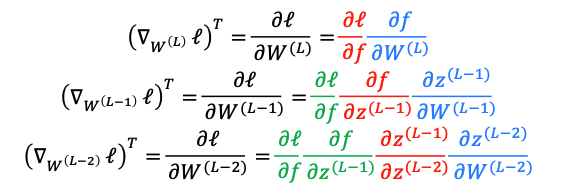
\includegraphics[width=\columnwidth]{jo/backpropagation.png} \\[-10pt]

Only compute \textbf{the gradient}. Rand. init. weights by distr. assumption for $\varphi$. ( $2 / n_{in}$ for ReLu and $1/n_{in}$ or $ 1/ (n_{in} + n_{out})$ for Tanh)

\subsection*{Gradient Descent, i.o.i}
Converges only for convex case. $\mathcal{O}(n * k * d)$
$$
	w^{t+1} = w^t - \eta_t \cdot \nabla \ell(w^t)
$$

For linear regression:
$$
	||w^t - w^*||_2 \leq ||I - \eta X^\top X||_{op}^t ||w^0 - w^*||_2
$$

$\rho = ||I - \eta X^\top X||_{op}^t$ conv. speed for const. $\eta$. Opt. fixed $\eta = \frac{2}{\lambda_{\text{min}} + \lambda_{\text{max}}}$ and max. $\eta \leq \frac{2}{\lambda_{\text{max}}}$. 

\textbf{Momentum}: $w^{t+1} = w^t + \gamma \Delta w^{t-1} - \eta_t \nabla \ell(w^t)$
Learning rate $\eta_t$ guarantees convergence if $\sum_t \eta_t = \infty$ and $\sum_t \eta_t^2 < \infty$

\section{Graphics Pipeline}

\begin{compactenum}
        \item Modelling Transform (Object to World Space)
        \item Viewing Transform (World to Camera Space)
        \item Primitive Processing (Output primitives from transformed vertices)
        \item 3D-Clipping (Remove primitives outside the frustum)
        \item Screen-Space Projection (Project from 3D to 2D screen space)
        \item Scan Conversion (Discretize continuous primitives)
        \item Lighting, Shading, Texturing
        \item Occlusion Handling (Update Color using Z-buffer)
        \item Display
\end{compactenum}
\greenbf{Programmer's View:} \\
%\includegraphics*[width = \columnwidth]{arjun/pipeline-programmer.png} \\
\includegraphics*[width = \columnwidth]{jo/rasterization.png} \\
\greenbf{Vertex Processing:} Per-vertex operations e.g Transforms and Lighting flow control. This is done with the Vertex Shader.  Input: uniforms and per-vertex attributes. Output: Varying per vertex\\
\greenbf{Fragment Processing:} Per-fragment operations e.g. Shading and Texturing Blending. This is done with the Fragment Shader. Input: Uniform and varying per-fragment attributes. Output: Per-fragment color\\
\greenbf{Inputs/Outputs:}
\begin{compactitem}
    \item Uniforms: (V/F) global constant inputs e.g. light position, texture map etc.
    \item Varying: (V/F) value passed from vertex to fragment shader by being interpolated across primitives first. e.g interp. pixel color
\end{compactitem}



\section{Colors and Light}
\greenbf{CIE Experiment:} subject is shown two stimuli at the same time, one with the pure spectral color, the other a linear combination of the three primaries (RGB). Subject can control how much primaries were dimmed and asked to match the second stimulus to the first. $\rightarrow$ find how humans perceive color. Can also add red light to reference if impossible to match $\rightarrow$ negative red values. \\
\greenbf{xyY color space:} x,y control chormacity, Y is luminance. 
\begin{wrapfigure}[9]{l}{0.4\columnwidth} %changing the dimensions will mess everything up so be careful!!
    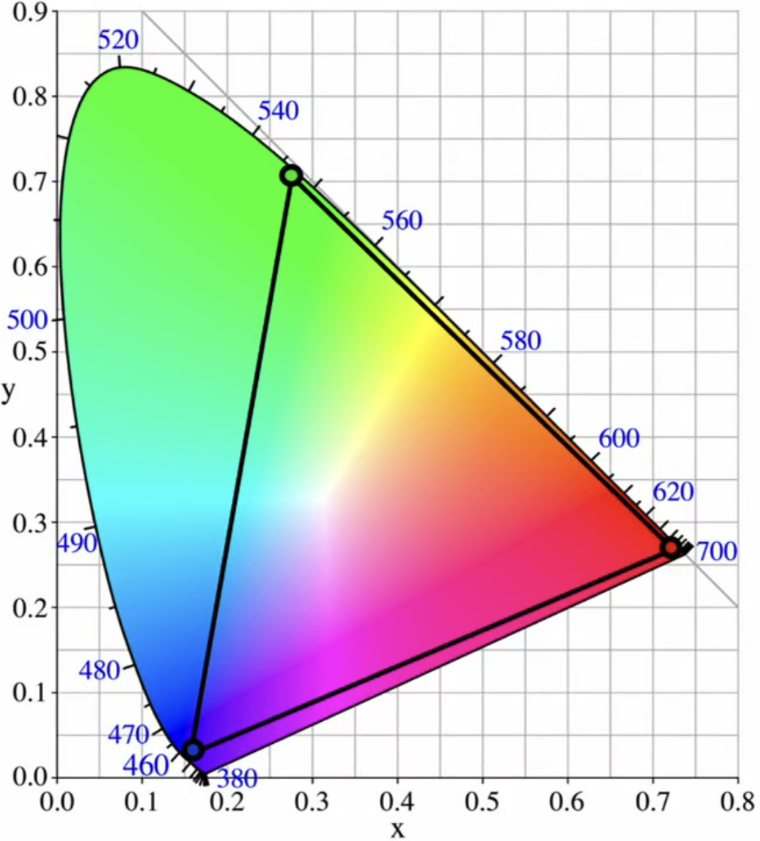
\includegraphics[width=0.4\columnwidth]{arjun/cie-chromacity.png}
\end{wrapfigure}
\greenbf{White point:} $(x,y) = (0.3,0.3)$ \\
\greenbf{Purple line:} Line connecting 380 and 770mm of non-spectral colors. \\
\greenbf{Isoline:} a line with about constant distance to the border \\
\greenbf{Inverse color:} Intersection of line drawn by the color and white point with the opposite border. 
\greenbf{xyY to XYZ:} 
$X = x \frac{Y}{y} \quad Z = \frac{Y}{y} - x \frac{Y}{y} - Y$

\greenbf{XYZ to xyY:}
$x = \frac{X}{X + Y + Z} \quad y = \frac{Y}{X + Y + Z}$

\greenbf{RGB:} Same color space as XYZ. Can be transformed with matrix multiplication. Additive color model, good for combining colored lights. Used in monitors/displays. \\
\greenbf{CMY:} Inverse of RGB. Subtractive color model. Used in passive color systems (printers). \\
\greenbf{RGB to CMY:} 
$\begin{bmatrix}
    \begin{smallmatrix}
        R \\ G \\ B
    \end{smallmatrix}
\end{bmatrix} = 
\begin{bmatrix}
    \begin{smallmatrix}
        1 \\ 1 \\ 1
    \end{smallmatrix}
\end{bmatrix} - 
\begin{bmatrix}
    \begin{smallmatrix}
        C \\ M \\ Y
    \end{smallmatrix}
\end{bmatrix}$ \\
\greenbf{YIQ:} Luminance Y, In-phase I (orange-blue), Quadrature Q (purple-green) components. Advantages for natural and skin colors. Used in NTSC US-color TV. \\
\greenbf{HSV:} Hue: base color, Saturation: purity of color, Value: brightness. Intuitive for interactive color picking. Used by designers.
\section{Transformations}
\greenbf{Linear functions:}
$f(ax + by) = af(x) + bf(y)$

\greenbf{Homogeneous Coordinates:} Raise dimensionality by 1 and set its coordinate to 1. 
\begin{center}
$
\begin{pmatrix}
    %\begin{smallmatrix} 
        x & y 
    %\end{smallmatrix} 
\end{pmatrix}^T \leftrightarrow 
\begin{pmatrix}
    %\begin{smallmatrix} 
        xw & yw & w 
    %\end{smallmatrix} 
\end{pmatrix}^T
w \in \mathbb{R}\backslash\{0\}
$
\end{center}
This allows non-linear transformations to still be denoted as matrices. \\
\greenbf{Translation:}
    $\begin{bmatrix}
        %\begin{smallmatrix}
            1 & 0 & t_x \\
            0 & 1 & t_y \\
            0 & 0 & 1
        %\end{smallmatrix}
    \end{bmatrix}$
\greenbf{Scale:}
$\begin{bmatrix}
    %\begin{smallmatrix}
        s_x & 0 & 0 \\
        0 & s_y & 0 \\
        0 & 0 & 1
    %\end{smallmatrix}
\end{bmatrix}$ \\
\greenbf{Rotations:}
Not commutative. $R^{-1} = R^T$. \\
3D-rotate(x):
$\begin{bmatrix}
    %\begin{smallmatrix}
        1 & 0 & 0 & 0 \\
        0 & cos(\theta) & -sin(\theta) & 0 \\
        0 & sin(\theta) & cos(\theta) & 0\\
        0 & 0 & 0 & 1
    %\end{smallmatrix}
\end{bmatrix}$\\
3D-rotate(y):
$\begin{bmatrix}
    %\begin{smallmatrix}
        cos(\theta) & 0 & sin(\theta) & 0 \\
        0 & 1 & 0 & 0 \\
        -sin(\theta) & 0 & cos(\theta) & 0\\
        0 & 0 & 0 & 1
    %\end{smallmatrix}
\end{bmatrix}$\\
3D-rotate(z):
$\begin{bmatrix}
    %\begin{smallmatrix}
        cos(\theta) & -sin(\theta) & 0 & 0 \\
        sin(\theta) & cos(\theta) & 0 & 0 \\
        0 & 0 & 1 & 0\\
        0 & 0 & 0 & 1
    %\end{smallmatrix}
\end{bmatrix}$\\
To rotate around arbitrary axes, see Quaternions. 

\greenbf{Shear:}\\
$
\begin{bmatrix}
    \begin{smallmatrix}
    1 & 0 & sh_x & 0 \\
    0 & 1 & sh_y & 0 \\
    0 & 0 & 1 & 0 \\
    0 & 0 & 0 & 1
    \end{smallmatrix}
\end{bmatrix}
$$
\begin{bmatrix}
    \begin{smallmatrix}
    1 & sh_x & 0 & 0 \\
    0 & 1 & 0 & 0 \\
    0 & sh_z & 1 & 0 \\
    0 & 0 & 0 & 1
    \end{smallmatrix}
\end{bmatrix}
$$
\begin{bmatrix}
    \begin{smallmatrix}
    1 & 0 & 0 & 0 \\
    sh_y & 1 & 0 & 0 \\
    sh_z & 0 & 1 & 0 \\
    0 & 0 & 0 & 1
    \end{smallmatrix}
\end{bmatrix}
$\\
\greenbf{Rigid Transformation:} 
Transformation that preserves vector length. (Only rotation \& translation)

\greenbf{Change Coordinate Systems: }

$p' = \begin{bmatrix}
    \mathbf{r_1} & \mathbf{r_2} & \mathbf{r_3} & \mathbf{t} \\
    0 & 0 & 0 & 1
\end{bmatrix}p$ where $\mathbf{r_1},\mathbf{r_2},\mathbf{r_3}$ are the old axes in the new system and $\mathbf{t}$ is the translation from new origin to old origin. \\
Transform normals with:\\
$p' = Mp \Rightarrow n' = (M^{-1})^Tn$

\subsection*{Quaternions}
Rotations and translations efficiently. 
\begin{center}
   $z = a + bi + cj + dk$\\
    $\begin{pmatrix}
    u & v & w
    \end{pmatrix}^T \leftrightarrow 0 + ui + vj + wk$
\end{center}
\greenbf{Properties:}
$i^2 = j^2 = k^2 = -1 \quad ijk = -1 \\ ij = k \quad ki = j \quad jk = i \\ ji = -k \quad ik = -j \quad kj = -i$\\
\greenbf{Vector form:} $z = s + \mathbf{v} \quad$ \textbf{v} is a vector, s is a scalar\\
\greenbf{Product:} $(s_1 + v_1) \cdot (s_2 + v_2) = s_1s_2 - v_1 \cdot v_2 + s_1v_2 + s_2v_1 + v_1 \times v_2$\\
\greenbf{Conjugate:} $\overline{(s_1 + v_1)} = s_1 - v_1, \quad z\overline{z} = \lVert z \rVert ^2 $\\
\greenbf{Inverse:} $z^{-1} = \frac{\overline{z}}{\lVert z \rVert ^2}, \quad 1 = z^{-1}z = zz^{-1} $\\
\greenbf{Rotation:} Vector $a = (x, y, z)^T$, rotate around $u$
\begin{compactenum}
    \item $(x,y,z)^T \rightarrow $ Quaternion $p = 0 + xi + yj + zk$
    \item Compute $q = cos(\frac{\theta}{2}) + sin(\frac{\theta}{2})\frac{u}{\lVert u \rVert}$ and $q^{-1} = \overline{q}$
    \item $p' = qpq^{-1}$
\end{compactenum}
    

\section{Shading and Lighting}
\greenbf{Flux:} $\Phi(A) [\frac{J}{s} = W]$ total energy/photons passing through space A per time unit.\\
\greenbf{Radiosity:} $B(x) = \frac{d\Phi(A)}{dA(x)} [\frac{W}{m^2}]$ Flux per unit area leaving surface \\
\greenbf{Irradiance:} $E(x) = \frac{d\Phi(A)}{dA(x)}[\frac{W}{m^2}]$ Flux per unit area arriving at surface\\
\greenbf{(Rad.) Intensity:} $I(\overrightarrow{\omega}) [\frac{W}{sr}]$ Flux per solid angle emanating from point source\\
\greenbf{Radiance} $L(x, \overrightarrow{\omega}) = \frac{d^2 \Phi(A)}{cos\theta dA(x) d\overrightarrow{\omega}} [\frac{W}{m^2 sr}]$ Intensity per unit area
\subsection*{BRDF}
Bidirectional Reflectance Distribution Function encodes behavior of light that bounces off a surface, given incoming direction $\omega_i$, how much gets reflected in outgoing direction $\omega_o$. \\
\greenbf{Reflection function:} \\
$f_r(x,\overrightarrow{\omega_i}, \overrightarrow{\omega_r}) = \frac{dL_r(x, \overrightarrow{\omega_r})}{L_i(x, \overrightarrow{\omega_i}) cos \theta_i d\overrightarrow{\omega_i}}$ \\
$\omega_i$ is the incoming light vector, $\omega_r$ the reflected. $\theta_i$: angle of incoming vector to the surface normal. \\
$f_r$ is constant for diffuse reflections.
\greenbf{Reflection Equation:} Reflected radiance due to illumination from all directions. \\
$L_r(x, \overrightarrow{\omega_r}) = \int_{H^2} f_r(x, \overrightarrow{\omega_i}, \overrightarrow{\omega_r})L_i(x, \overrightarrow{\omega_i}) cos \theta_i d \overrightarrow{\omega_i}$ \\
For diffuse reflections, $f_r$ is constant. \\
$L_r(x) = f_r E_i(x) = f_r \int_{H^2}L_i(x, \overrightarrow{\omega_i}) cos \theta_i d \overrightarrow{\omega_i}$





\greenbf{Types of reflections:}\\
\includegraphics*[width = \columnwidth]{arjun/light-reflections.png}
Additionally there is also retro-reflective, which reflects the light back to the source in a way similar to glossy. 

\subsection*{Phong Illumination Model}
This is a local illumination model: does not consider indirect light bouncing of from others objects that are hitting the object, unlike the global illumination model. It is approximated by ambient lighting.
Light shines into the surface but is viewed as an outgoing vector in the model.\\
\greenbf{Ambient:} Light that shines independent of viewpoint \& angle. (Imagine it as object glowing) \\
\greenbf{Diffuse:} General direction of the light which is reflected regardless of viewer's position.\\
\greenbf{Specular:} Shiny light reflection
$$I = \underbrace{I_ak_a }_\text{Ambient} + I_p \bigl( \underbrace{k_d(N \cdot L)}_\text{Diffusion} + \underbrace{k_s(R \cdot V)^n}_\text{Specular} \bigr)$$
The material parameters are $k_a, k_d, k_s, n$. $I_a, I_p$ are light intensities, $N$ normal surface, $L$ the light ray, $R$ the reflection ray, and $V$ the viewing ray. $R, V, L, N$ are all normalised. 

\begin{minipage}{0.6\columnwidth}
    $R = \frac{2(N \cdot L)N - L}{\lVert R \rVert} $ \\
$V = \frac{Eye position - Object position}{\lVert V \rVert} $
\end{minipage}
\begin{minipage}{0.4\columnwidth}
    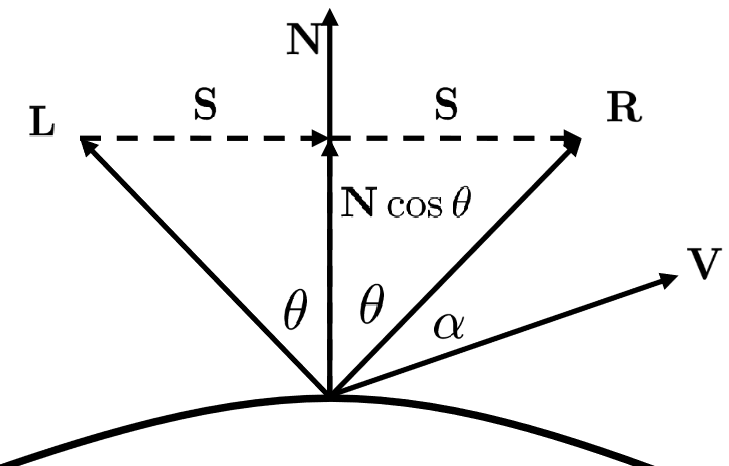
\includegraphics[width = \linewidth]{arjun/phong-illumination.png}
\end{minipage}
\greenbf{Attenuation}
    Quadratic due to spatial radiation. \(f_{att} = (d_L^2)^{-1}\) or often used in OpenGL:
    \(f_{att} = \min((c_1 + c_2d_L + c_3d_L^2)^{-1}, 1)\)
  
  
  \greenbf{Cook-Torrence}
    For metal objects which replaces the specular term. Has self-shadowing effects.
  
  
  \greenbf{Ashikhmin}
    Anisotropic lighting model.
  
\subsection*{Shading}
\greenbf{Flat:} 1 color per primitive, per triangle \\
\greenbf{Gouraud:} Linearly interpolate vertex intensities
\begin{compactenum}
    \item Calculate vertex normal by averaging face normals.
    \item Evaluate illumination model for each vertex
    \item Interpolate vertex colors bilinearly on the scan line.
\end{compactenum}
\begin{center}
    \includegraphics*[width = 0.5\columnwidth]{arjun/gouraud-shading.png}
\end{center}

$I_a = I_1 - (I_1 - I_2)\frac{(y_1-y_s)}{(y_1 - y_2)}$  
$I_b = I_1 - \left(I_1 - I_3\right) \frac{\left(y_1 - y_s\right)}{\left(y_1 - y_3\right)}$ 
$I_p = I_b - \left(I_b - I_a\right) \frac{\left(x_b - x_p\right)}{\left(x_b - x_a\right)}
$

Problems: Perspective Distortion. Orientation Dependence due to interpolation. Shared Vertices.

\greenbf{Phong Shading:} Linearly interpolate normals, color per pixel, problem: normal not defined/representative
\begin{compactenum}
    \item Calculate vertex normal by averaging face normals.
    \item Interpolate the normal barycentric
    \item Evaluate illumination model per fragment in triangle
\end{compactenum}
\begin{center}
    \includegraphics*[width = 0.5\columnwidth]{arjun/phong-shading.png}
\end{center}

$ n_x = \lambda_an_a + \lambda_bn_b + \lambda_cn_c  \quad \lambda_a = \frac{\color{blue} \Delta xbc}{\Delta abc} \quad \lambda_b = \frac{\color{red} \Delta xac}{\Delta abc} \quad \lambda_c = 1 - \lambda_a - \lambda_b$ 

\subsection*{Transparency}
\greenbf{Alpha Blending:} is the linear interpolation of color front-to-back (obj. 1 is closer than obj. 2): $I = I_1 \alpha_1 + \alpha_2 I_2 (1 - \alpha_1)$\\
$\alpha = 1 $: opaque. $\alpha = 0$: transparent.\\
We render back to front, beginning with opaque object. Can cause issues with overlapping objects. Solution is depth peeling. We do multiple passes where each pass renders the next closest fragment.
\section{Geometry \& Textures}
\greenbf{Challenges, texture:} Noisy captured images, visual redundancy over space, callibration inaccuracies, reconstruction inaccuracies, occlusions, visual redundancy over time geometric noise \graytext{(reconstruction noise \& callibrating noise)}\\
\greenbf{Ways to encode geometry:} \\
Explicit: Vertex positions are given explicitly $\rightarrow$ good for sampling, bad for testing whether inside or outside object.\\
Implicit: Vertex positions fulfil some equation. $\rightarrow$ good to test inside/outside object, compact description, tough to model complex shapes, finding all points is expensive.\\
\greenbf{Geometry representations implicit}\\
%\begin{compactitem}
    Parametric surfaces: \graytext{surfaces defined by parameter space}\\
    Algebraic surfaces: \graytext{surface is zero set of pol.}\\
    Constructive solid geometry: \graytext{compl. shapes}\\
    Blobby surfaces: \graytext{blend surfaces toget.}\\
    Blending distance func.: \graytext{distance to closest p. on object}\\
    Level set methods: \graytext{grid of values approx. func.}\\
    Fractals and L-systems: \graytext{self-similar}\\
%\end{compactitem}
\greenbf{Geometry representations explicit}\\
%\begin{compactitem}
    Point set: \graytext{collection of p. can be combined to surf.}\\
    Point cloud: \graytext{list of points $(x, y, z)$}\\
    Polygonal mesh: \graytext{easier processing simulation, common}\\
    Triangle mesh, Subdivision surfaces: \graytext{smooth out a control curve, insert new vertex at each edge midpoint and update vertex positions according to fixed rule}
 %\end{compactitem}

\subsection*{Mesh Datastructure}
\greenbf{Triangle List:} List containing ($v_1, v_2, v_3$) where $v_i$ is the coordinates $\Rightarrow$ easy query, but redundant.\\
\greenbf{Indexed Face Set:} List containing vertex ids and another list of vertices with their coordinates $\Rightarrow$ less storage space.
\subsection*{Polygonal Mesh} Set of connected polygons where every edge belongs to at least one polygon and the intersection of two polygons either empty, a vertex or and edge.\\
\greenbf{Manifolds:} surface homeomorphic to a disk, closed manifolds divides space into two.

\subsection*{Texture Mapping}
Enhance details without increasing geometric complexity. Desirable properties: low distortion, bijective mapping, efficiency. \\
\greenbf{Parametrization:} Map $(u,v)$ coordinates of texture to 3D vertex coordinates. E.g. for spheres
$\begin{bmatrix}
    \begin{smallmatrix}
        u \\ v
    \end{smallmatrix}    
\end{bmatrix} \mapsto 
\begin{bmatrix}
    \begin{smallmatrix}
        sin(u)sin(v) \\
        cos(v)\\
        cos(u)sin(v)
    \end{smallmatrix}
\end{bmatrix}$\\
\greenbf{Texture Filtering:} To prevent aliasing, we should apply low pass filter to the texture. \\
\greenbf{Maps:}
\begin{compactitem}
    \item Light map: simulates effect of a local light source
    \item Environment map: render reflective object efficiently
    \item Bump mapping
    \item Normal mapping
    \item Mipmapping
\end{compactitem}
\greenbf{Bump Mapping:}
Perturbs surface normal. Encodes height difference (grayscale) from mesh. Illusion of geometry, but (self-)shadows and silhouette unchanged. \\
\greenbf{Normal mapping:}
Very similar to bump mapping but now stored as $(r,g,b)$ color $\Rightarrow$ directional perturbations. More detailed \\
\greenbf{Mipmapping:}
Store down-sampled versions of a texture using Gaussian Pyramid. Choose resolution based on projected size of triangle. Use linear interpolation between resolutions. Prevents aliasing!\\
\greenbf{Magnification:}
Pixel in texture image maps to area larger than one pixel $\rightarrow$ Jaggies. Can be solved by bilinear interpolation. \\
\greenbf{Minification:}
Pixel in texture image maps to area smaller than one pixel $\rightarrow$ moiré patterns. Solution: mipmapping.
\section{Signal Processing}

%\section{Drawing Triangles}
\blindtext
%\section{Transform Geometry and Textures}
\blindtext

\section{Scan Conversion}
\greenbf{Scan Conversion / Rasterisation:} Convert vector-based/geometric objects into pixel-based images. Crucial for rendering graphics on computer screens. \\ 
\greenbf{Bresenham Line:}
Choose closest point at each intersect with vertical pixel grid lines. \\
\textbf{Implicit line equation:} $f(x,y) = ax + by + c = 0$;\\
\textbf{Last colored pixel:} \\
$p = (x_p, y_p)$; $d = f(m) = f(x_p + 1, y_p + 1/2)$;\\
If $d < 0$ select lower pixel E else if $d > 0$ select upper pixel NE. \\
For next pixel, \\
\textbf{Case E:} $d_{new} = f(x_p + 2, y_p + 1/2) = a + d = d + \delta{y}$; \\
\textbf{Case NE:} \\
$d_{new} = f(x_p + 2, y_p + 3/2) = a + b + d = d + \Delta{y} - \Delta{x}$

\greenbf{Scan Conversion for Polygons:} 
\begin{compactitem}
    \item Most important graphics primitive
    \item CPU can process up to 50 mil triangles/s
    \item Straightforward approach: inside test for every pixel but instead process scan-line after scan-line
\end{compactitem}
\greenbf{Algorithm}
\begin{compactenum}
    \item Calculate all intersections on a scan-line
    \item Sort intersections by ascending x-coordinates
    \item Fill all spans in between two consecutive intersection points if parity is odd
\end{compactenum}

\section{Bézier/Hermite Curves}
\greenbf{Spline desired properties:} \\
Interpolation: \graytext{Spline passes exactly through data points}\\
Continuity: \graytext{in $C^2$}\\
Locality: \graytext{moving one point does nto affect whole curve} \\
$\implies$ impossible to have all at once
Cubic polynomials, interpolate + 1st derivate is given tangent. Interpolates, not $C^2$-continuous, local
\greenbf{Maps:} $\mathbb{R}^1 \to \mathbb{R}^3$ : $x(u) = (x(u), y(u), z(u))^T$, $\mathbb{R}^2 \to \mathbb{R}^3$ : $x(u,v) = (x(u,v), y(u,v), z(u,v))^T$
\greenbf{Bezier Curves:}
${x}(t) = b_0 B_0^n(t) + \dots + b_n B_n^n(t)$ where $b_0 ...b_n$ are the control points. 
\\
$n = 3 $ : ${x}(t) = b_0(1-t)^3 + 3b_1t(1-t)^2 + 3b_2t^2(1-t) + b_3t^3$. 
\\
\textbf{Derivative:} $\frac{d}{dt} b^n(t) = n \sum_{i=0}^{n} \left( B_{i-1}^{n-1}(t) - B_i^{n-1}(t) \right) b_i$, which is a Bezier curve with degree $n - 1$\\
\textbf{Properties:} design property: control points give rough sketch, endpoint interpolation, variation diminishing property: intersection of straight line with curve $<=$ \# control points.\\
\textbf{Disadvantages:} global support of basis functions (changing one control point changes entire curve), inserting control points expensive, lack of continuity between different segments\\
\greenbf{Bernstein Polynomial of degree n:}
$B_i^n(t) = \binom{n}{i} t^i (1 - t)^{n-i} \text{ for } 0 \leq i \leq n$ zero else. 
\\
Global support, positive definite, partition of unity, different degrees. 
\\
Derivative: $\frac{d}{dt} B_i^n(t) = n \left( B_{i-1}^{n-1}(t) - B_i^{n-1}(t) \right)$


\greenbf{Binomial coefficient:}\\
$\binom{n}{i} = \frac{n!}{i!(n-i)!} \text{for } 0 \leq i \leq n$ zero else.

\greenbf{DeCasteljau Algorithm:}
Recursive method for computing a point on a bezier curve using a systolic array in O($n^2$):
Given \( n+1 \) control points \( b_0, b_1, \ldots, b_n \) the recursion is defined as follows:
\begin{align*}
b_i^r(t) &= (1 - t) b_i^{r-1}(t) + t b_{i+1}^{r-1}(t) \\
b_i^0(t) &= b_i \\
&\text{for } r = 1, \ldots, n \text{ and } i = 0, \ldots, n-r
\end{align*}
Intuition: Corner cutting until only one line remains whose intersection with the curve is the result. 

\greenbf{Forward difference operator $\Delta:$} $\Delta b_j = b_{j+1} - b_j$
Bezier curve derivative with $\Delta$: \\ $\frac{d}{dt}b^n(t) = n\sum_{j=0}^{n-1} \Delta b_j \cdot B_i^{n-1}$


\greenbf{Recursive $\Delta^r$:} \\
\textbf{recursive:} $\Delta^r b_j = \Delta^{r-1}b_{j+1} - \Delta^{r-1}b_j$\\
\textbf{non-recursive:} $\Delta^r b_i = \sum_{j=0}^r \binom{r}{j} (-1)^{r-j} b_{j+i}$\\
\textbf{Higher order derivative of Bezier curve:} $\frac{d^r}{dt^r} b^n(t) = \frac{n!}{(n-r)!} \sum_{j=0}^{n-r} \Delta^r b_j B_j^{n-r}(t)$\\
\greenbf{Piecewise Bezier Curves / Splines:}\\
Knots: $u_0 < ... <u_L$, \\
Intervals: $[u_i, u_{i+1}]$, \\
local parameter: $t = \frac{u - u_i}{u_{i+1} - u_i} = \frac{u - u_i}{\Delta_i}$. \\
Segment $s(u) = s_i(t)$, \\
a Bezier curve that is a function of the local parameter t.
$\frac{ds(u)}{du} = \frac{ds_i(t)}{dt}\frac{dt}{du} = \frac{1}{\Delta_i}\frac{ds_i(t)}{d_t}$. \\
\textbf{Enforce Continuity:} Curve in $[u_0, u_2]$ decomposed to bezier segments $b_0, ..., b_n$ in $[u_0, u_1]$ and $b_n, ..., b_{2n}$ in $[u_0, u_1]$, $C^r-Continous$ if $b_{n+1} = b_{n-i}^i(t)$ for $i = 0,...,r$ and $t = \frac{u - u_0}{u_1 - u_0 }$. $C^1-Continuity$: Control points $b_n-1, b_n, b_{n+1}$ are colinear. 

\greenbf{Matrix form:} $x(t) = \sum_{i=0}^nc_iC_i(t)$. Basis transform into monomial representation with $M=\{m_{ij}\}$:
$
\begin{bmatrix}
C_0(t) \\
\vdots \\
C_n(t)
\end{bmatrix}
=
\begin{bmatrix}
m_{00} & \cdots & m_{0n} \\
\vdots & \ddots & \vdots \\
m_{n0} & \cdots & m_{nn}
\end{bmatrix}
\begin{bmatrix}
t^0 \\
\vdots \\
t^n
\end{bmatrix}
$
\\
For Bernstein: $m_{ij} = (-1)^{j-i} \binom{n}{j} \binom{j}{i}$
\\
\greenbf{Spline interpolation:} Interpolate a set of points $p_0, ..., p_n$ using basis functions. For monomials as basis: $p_i = x(t_i) = \sum_{j=0}^{n} a_j(t_i)^j, \quad i \in [0,n]$. Resulting in Vandermonde matrix (ill-conditioned): 
$
\begin{bmatrix}
1 & t_0 & \cdots & t_0^n \\
\vdots & \vdots & \ddots & \vdots \\
1 & t_n & \cdots & t_n^n
\end{bmatrix}
\begin{bmatrix}
a_0 \\
\vdots \\
a_n
\end{bmatrix}
=
\begin{bmatrix}
p_0 \\
\vdots \\
p_n
\end{bmatrix}
$

\greenbf{Blossoming:} Generalisation of deCasteljau. TODO

\section{B-Spline Curves}
not interpolating, $C^2$-continuous, local
How many knots does a knot vector need to have?: $k + n + 2$ where $k = $ degrees of freedom\\
\greenbf{B-Spline:} $s(u) = \sum_{i=0}^kd_iN_i^n(u)$ with deBoor points $d_i$ and knot vector $u = [u_0, ..., u_{k+n+1}]$ (k is degree of freedom and n polynomial degree).\\ 
\textbf{Recurrence:} Recurrence relation: $N_i^n(u) = \frac{(u - u_i)}{u_{i+n} - u_i} N_i^{n-1}(u) + \frac{(u_{i+n+1} - u)}{u_{i+n+1} - u_{i+1}} N_{i+1}^{n-1}(u)$, where $N_i^0(u) = \begin{cases} 1, & u \in [u_i, u_{i+1}) \\ 0, & \text{else} \end{cases}$. B-Spline bases of degree has support over $n+1$ intervals of the knot vector.\\
\textbf{B-Spline filters:} Widely used in signal processing. Cardinal B-Splines over uniform knot sequences can be computed using the convolution operator: \( N_i^n = N^{n-1} * N^0 = \int_{0}^{x} N^{n-1}(t)N^0(x - t) dt \).\( N^0 \): box-function.\\
\textbf{Properties:} 
Partition of Unity: $\sum_i N_i^n(u) = 1$. 
Positivity: $N_i^n(u) \geq 0$.
Compact support: $N_i^n(u) = 0$, $\forall u \notin [u_i, u_{i+n+1}]$.
Continuity: $N_i^n$ is $(n-1)$ times continuously differentiable, if p knots overlap ($u_j = ... = u_{j+p-1})$ only $C^{n-p}$.
Variation diminishing property.
Convex hull property.


\greenbf{deBoor Algortihm:} We want to evaluate the B spline curve s(u) at point $u=t$. For given $t \in [u_I, u_{I+1}]$ all $N_i^n(u)$ vanish except for $i \in \{I-n, ...,I\}$. Point $s(t)$ computed by successive linear interpolation. Control point in $k$-th step: $d_i^k = (1 - a_i^k)d_{i-1}^{k-1} + a_i^k d_i^{k-1} $ where $ a_i^k = \frac{t - u_i}{u_{i+n+1-k} - u_i} $, $d_i^0 = d_i$, $d_n^n = s(t)$. Special case: If $0 = u_0 = ... = u_n < u_{n+1} = ... = u_{2n+1}$ with $u_{n+k} = 1$ for $k \in [1, ...,n+1]$ we get $d_i^k(u)=ud_i^{k-1}(u)+(1-u)d_{i+1}^{k-1}(u)$ (deCasteljau)

\greenbf{End Conditions:} How curve behaves at end points. For closed loop periodic deBoor points and knot vector: $d_0=d_{k++}, u_0=u_{k+1}$
\section{Tensor Product Surfaces}
2D to 2D mainly used for warping
No NURBS
\greenbf{Tensor Product Surface:} 2D/3D curve: $x(u) = \sum_{i=0}^mc_iF_i(u)$ with bases $F_i$ and coefficients $c_i$. For surfaces turn coefficients into functions of a second parameter: $c_i(v) = \sum_{j=0}^v\alpha_{i,j}G_j(v)$ resulting in the tensor product surface $x(u,v) = \sum_{i=0}^mc_i(v)F_i(u) = \sum_{i=0}^m\sum_{j=0}^n\alpha_{i,j}F_i(u)G_j(v)$

\greenbf{Bezier Patches:} Given bezier curve of degree m $b^m(u) = \sum_{i=0}^mb_iB_i^m(u)$ and control points $b_i$ as bezier curves of degree n: $b_i = b_i(v) = \sum_{j=0}^nb_{i,j}B_j^n(v)$ construct point on the surface: $b_{m,n}(u,v) = \sum_{i=0}^m\sum_{j=0}^nb_{i,j}B_i^m(u)B_j^n(v)$\\
\textbf{Properties:} affine invariance, convex hull, variation diminishing, boundary curves are bezier curves.

\greenbf{2D deCasteljau:} Algorithm for computing point on surface.

\greenbf{Warping:} Function from 2D to 2D, distorting an image

\greenbf{NURBS:} Non uniform rational b-splines. $\neq$  Tensor Product Surfaces since bases not separable. Top row: different B-splines, bottom row: nurb surface with different weigths
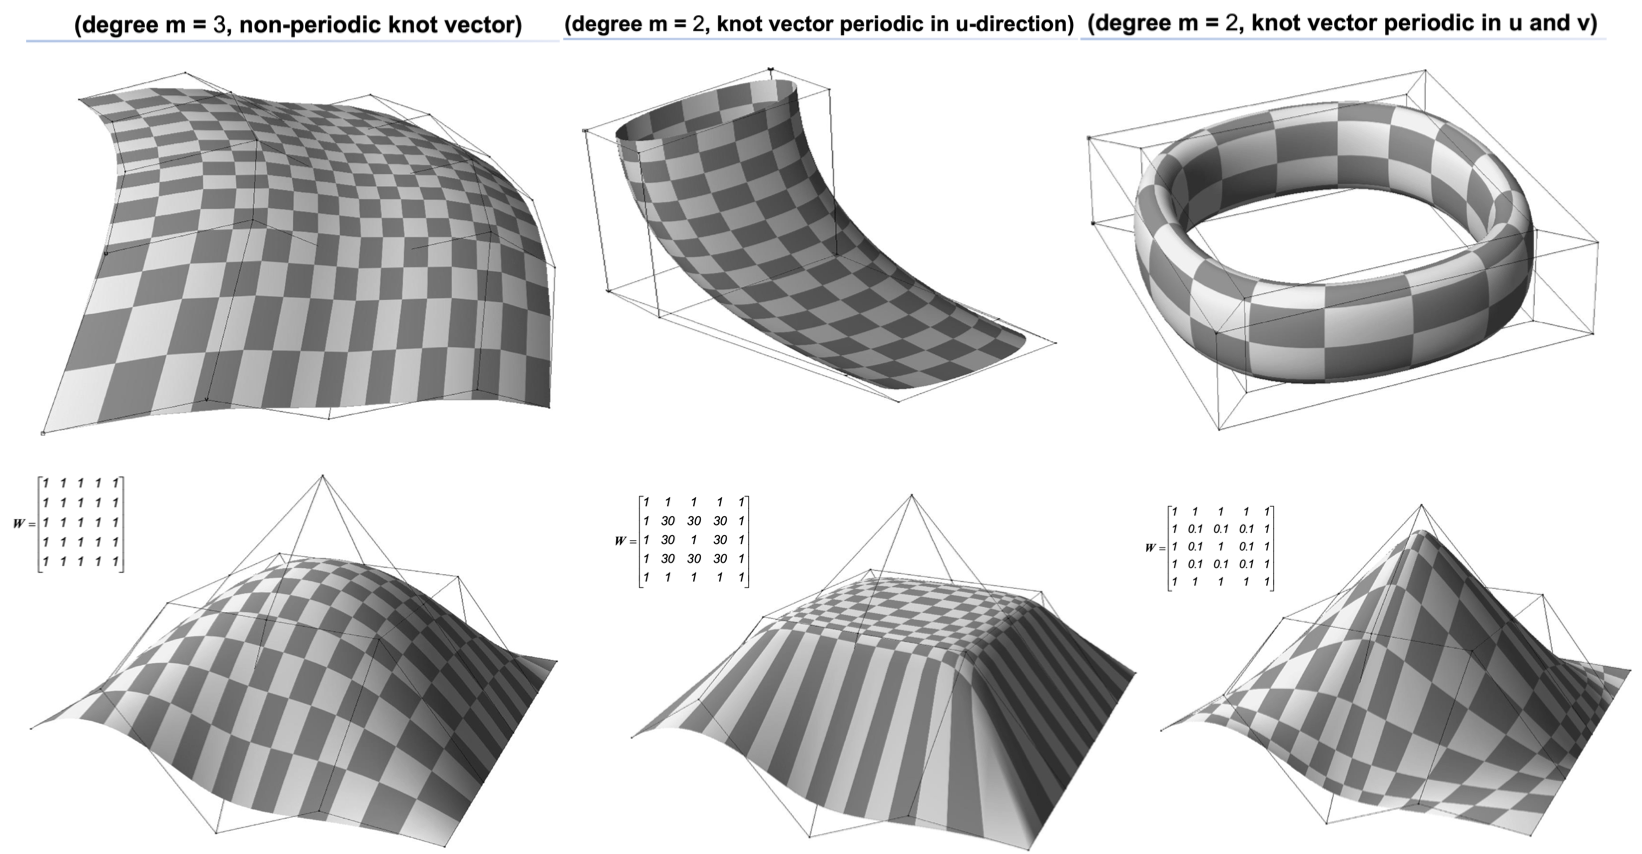
\includegraphics[width=\columnwidth]{assets/alex/bSplineSurfaces.png}
\section{Subdivision Surfaces}

\greenbf{Corner Cutting:} Insert two new vertices at $\frac{1}{4}$ and $\frac{3}{4}$ of each edge. Remove old and connect new vertices.
\includegraphics*[width = \columnwidth]{alex/cornerCutting.png}

\greenbf{Subdivision surfaces:} Generalisation of spline curves/surfaces, arbitrary control meshes, successive refinement, converges to smooth limit surface, connection between splines and meshes. In a sense similar to deCasteljau (corner cutting). No regular structure like curves (arbitrary number of edge neighbours, different subdivision rules for each valence). \\
\textbf{Classification:} Primal: faces are split into sub-faces. Dual: Vertices are split into multiple vertices. Approximating: Control points not interpolated. Interpolating: Control points interpolated.
\includegraphics*[width = \columnwidth]{alex/subdivisionClassification.png}
\greenbf{Geometric continuity:}  Weaker form of continuity focusing on the visual appearance, e.g. $G^n$ curve might be $C^{n-1}$ for a finite set of points and $C^n$ everywhere else.\\
\greenbf{Doo-Sabin:} 
\raisebox{-1ex}{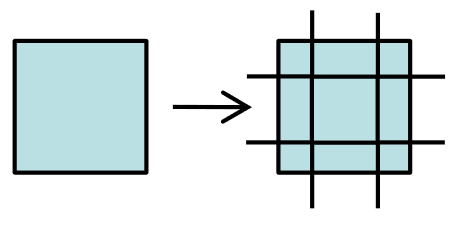
\includegraphics[height= 3ex]{assets/arjun/doo-sabin-icon.png}}
generalisation of bi-quadratic B-Splines, for polygonal meshes, generates $G^1$ continuous surfaces.\\
\greenbf{Catmull-Clark:} \raisebox{-1ex}{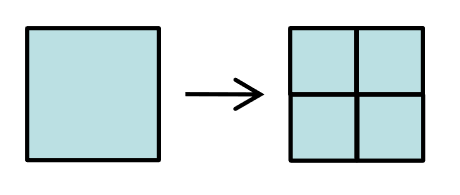
\includegraphics[height= 3ex]{assets/arjun/catmull-clark-icon.png}} generalisation of bi-cubic B-Spline, polygonal meshes, $G^2$\\
\greenbf{Loop Subdivision:} 
\raisebox{-1ex}{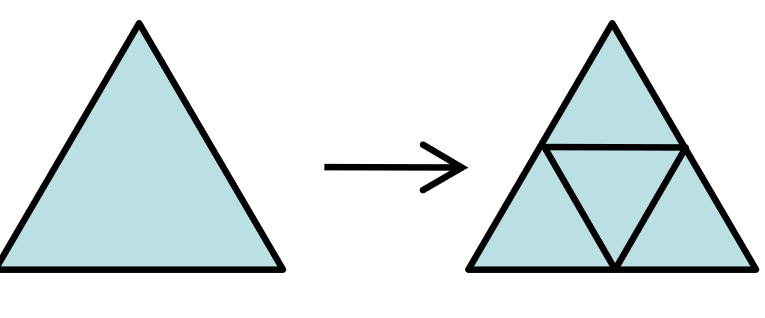
\includegraphics[height= 3ex]{assets/arjun/loop-subdivision-icon.png}} generalisation of box splines, triangle meshes, $G^2$\\
\greenbf{Butterfly:} triangle meshes, $G^1$ continuous\\
Top row: Start, Doo-Sabin, Catmull-Clark. \\
Bottom-row: Start, Loop Subdivision, Butterfly \\
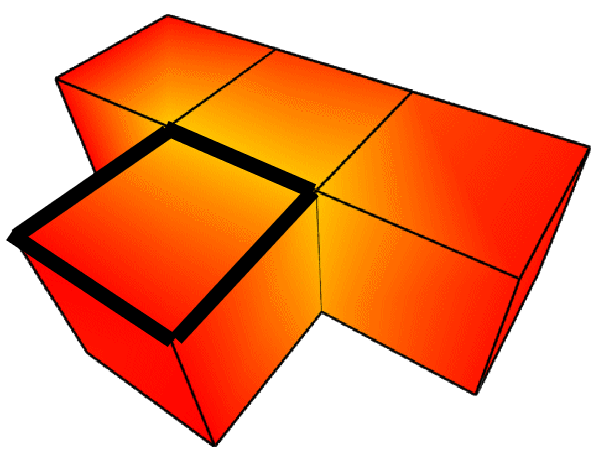
\includegraphics[width=0.3\columnwidth]{assets/arjun/start-square.png}
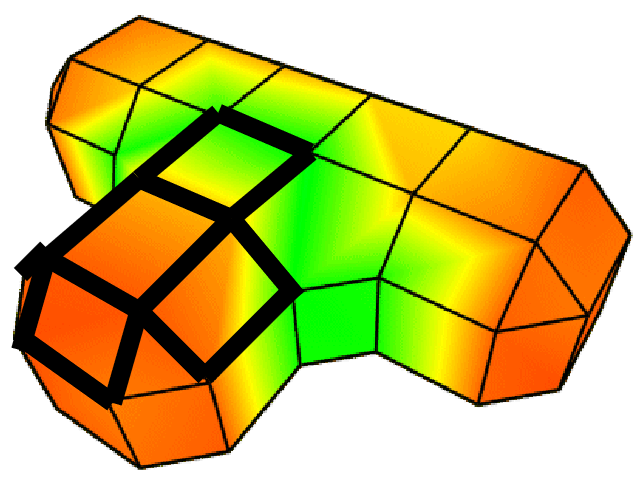
\includegraphics[width=0.3\columnwidth]{assets/arjun/doo-sabin.png}
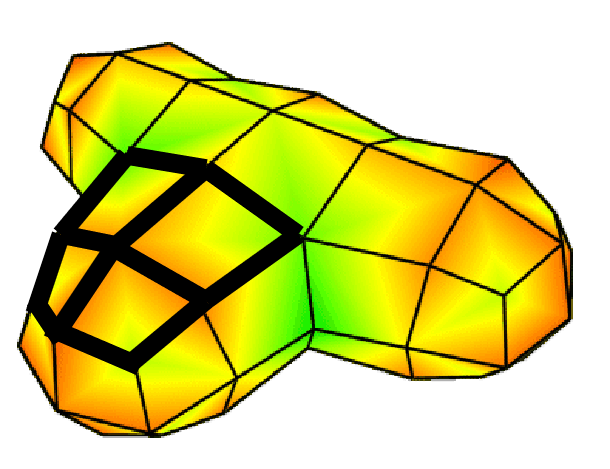
\includegraphics[width=0.3\columnwidth]{assets/arjun/catmull-clark.png}
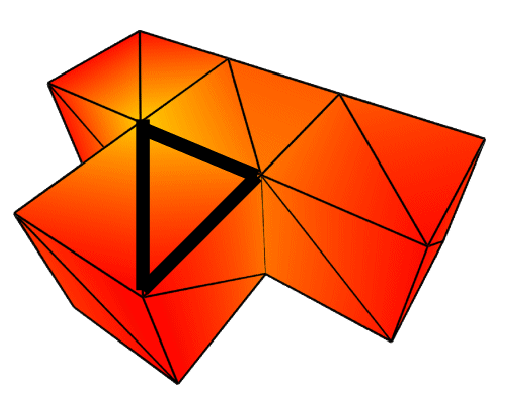
\includegraphics[width=0.3\columnwidth]{assets/arjun/start-triangle.png}
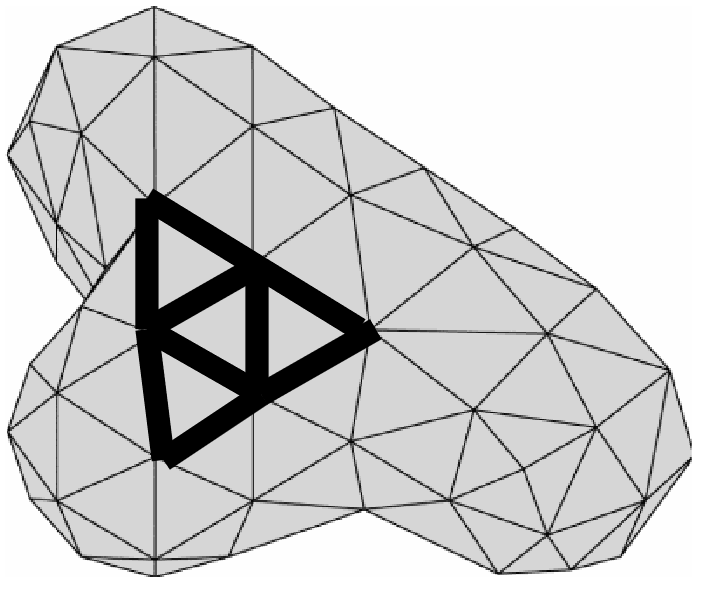
\includegraphics[width=0.3\columnwidth]{assets/arjun/loop-subdivision.png}
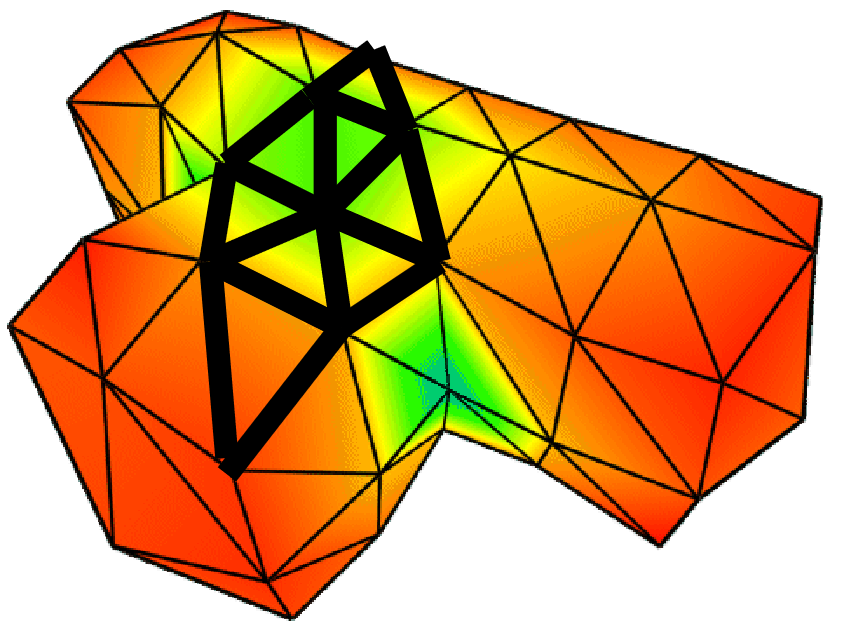
\includegraphics[width=0.3\columnwidth]{assets/arjun/butterfly.png}\\




\section{Visibility \& Shadows}

\greenbf{Visibility:} Some parts of of some surfaces are occluded by other surfaces.

\greenbf{Painter's Algorithm:} Render objects/Polygons from furthest to nearest. Problem: cyclic overlaps and intersections.

\greenbf{Z-Buffering:} Store depth to the nearest object for each pixel. 1.Initially all $\infty$. 2. For each Polygon, if the z value of a pixel for this polygon is smaller than the stored z value, replace the stored z value. Problems: limited resolution (only finite number of z values), non-linear (higher resolution for near objects, lower for far objects), setting near plane far from camera exacerbates resolution problem.

\greenbf{Shadows:} Important for perception of depth, realism, indicating light position and type (point light or area light).

\begin{center}
    \tiny
    \begin{tabularx}{\linewidth}{|X|X|X|X|X|}
        \hline
    \textbf{Feat/Limits} & \textbf{Plan. Fake Shad.} & \textbf{Proj. Texture Shad.}& \textbf{Shad. Maps} & \textbf{Shad. Vol.} \\
        \hline
        \textbf{Allows objects to cast shadows
        on themselves (self-shadowing)} & $\times$ & $\times$ & \checkmark & \checkmark \\
        \hline
        \textbf{Permits shadows on arbitrary
        surfaces (i.e. curved)} & $\times$ & \checkmark & \checkmark & \checkmark \\
        \hline
        \textbf{Generates extra geometric
        primitives} & $\times$ & $\times$ & $\times$ & \checkmark \\
        \hline
        \textbf{Limited resolution of
        intermediate representation can
        result in jaggy shadow artifacts} & $\times$ & \checkmark & \checkmark & $\times$ \\
        \hline
    \end{tabularx}
    \end{center}
    
\greenbf{Planar Shadows:} Draw projection of object on ground.

\greenbf{Projective texture shadows:} Separate obstacle (shadow caster) and receiver. Compute b/w image of the obstacle. Use image as projective texture map.

\greenbf{Shadow Maps:} Compute the depths from the light source and from the camera. Shadow map stores depths for light source. For each pixel on the camera plane compute the point $x$ in world coordinates consider its distance $z_L$ to the light source and $d(x_L)$ which is the depth in the direction: light source-x. If $d(x_L) < z_L$, x is in shadow. In order to prevent self-shadowing add bias: $d(x_L) < z_L + bias$, too small bias causes self shadows and to large bias removes too much shadow. In order to include points which are outside the FOV for the shadow map one can use cubical shadow maps. To prevent undersampling/aliasing take weighted average of "$d(x_L) + bias < z_L$" tests instead of filtering depth directly. Bigger filters give fake soft shadows, bias tricky


\greenbf{Shadow Volumes:} Explicitly represents the volume of space in shadow. If polygon is inside the volume, it is in shadow. Similar to clipping. Naive implementation: O(\#polygons * \#lights)\\
\textbf{Algorithm:}: 
\begin{compactitem}
    \item Shoot ray from eye.
    \item Incre-/decrement counter every time boundary of a shadow volume is intersected.
    \item If counter = 0 not in shadow.
\end{compactitem}
\textbf{Optimisation:} use silhouette edges only (where back-facing and front-facing polygon meet).\\
\textbf{Limitations:} introduces a lot of new geometry, expensive to rasterize long skinny triangles, objects must be watertight for silhouette optimisation, rasterization of polygons sharing and edge must not overlap or have gap.


\section{Ray Tracing}

\greenbf{Forward Ray Tracing:} light source $\to$ object $\to$ eye.

\greenbf{Backward Ray Tracing:} eye $\to$ object (secondary rays may be generated) $\to$ light source (in order to compute shadows). Basic pipeline: Ray-generation, Intersection, Shading, Repeat.

\greenbf{Ray generation:} pinhole camera???, Supersampling: multiple rays per pixel, prevents aliasing.

\greenbf{Ray-Surface Intersections:} For origin $o$ and direction $d$ ray: $r(t) = o + td$. For sphere with center $c$ and radius $r$ solve $\|r(t) - c\|^2 - r^2 = 0$ for t. For triangle with corners $p_1, p_2, p_3$ use barycentric coordinates $x = s_1p_1 + s_2p_2 + s_3p_3$, Intersect ray with triangle plane: $t = -\frac{(o-p_1)n}{dn}$ where $n = (p_2 - p_1) \times (p_3 - p_1)$, Compute $s_i$, test $s_1 + s_2 + s_3 = 1$ and $0 \leq s_i \leq 1$

\greenbf{Shading:} physically correct too costly, instead assume surface reflectance (diffuse, specular, ambient, transparent), use shadow rays for shadows. Extensions: model refraction,  multiple light sources, area light for soft shadows, sample and intersect in time for motion blur, depth of field.

\greenbf{Acceleration:} Cost for ray tracing O(\#rays * \#objects). \\
\textbf{Uniform grids}:
\begin{compactitem}
    \item Preprocess: Bounding box, grid resolution, rasterize objects, store references to objects. 
    \item Incrementally rasterize ray and stop at intersection with rasterized object. \\Advantages: fast to build, easy to code. 
    \\Disadvantages: not adaptive to scene geometry.
\end{compactitem}
\textbf{Space partitioning trees}: octree, kd-tree, bsp-tree.

%\section{Rendering Equation}
\blindtext
%\section{Rigging, FK and IK}
\blindtext
%\section{Partial Differential Equations}
\blindtext
%\section{Animation}
\blindtext
\section{OpenGL}
$\text{Resulting Col} = \\
\text{Src. Col.} \times \text{Src. Fac.} + \text{Dest. Col.} \times \text{Dest. Fac}$

projectionMatrix transforms points from camera space to screen space.

modelviewMatrix transforms points from object space to camera space.


\section{Radon Transformation}
The Radon transform $Rf(\theta, s)$ of a function $f(x, y)$ is defined as:\\
$
Rf(\theta, s) =\\
\int_{-\infty}^{\infty} \int_{-\infty}^{\infty} f(x, y) \delta(x\cos(\theta) + y\sin(\theta) - s) \,dx\,dy$

 $\theta$ is the angle of the projection, $ s $ is the distance parameter,
 $ \delta(\cdot) $ represents the Dirac delta function.


\greenbf{Properties}
\begin{compactitem}
    \item Linear
    \item Shifting only changes the \(\rho\) coordinate
    \item Rotation of the coordinate system also rotates the Radon transformation
    \item The Radon transform of a 2D convolution is a 1D convolution of the Radon transformed function with respect to \(\rho\)
\end{compactitem}

\greenbf{Reconstructing Image}

  Assume: attenuation of material in each px constant and \(\propto\) area of the px illuminated by the beam.
  \(k_{ij} = \frac{\text{are of pixel} \ j \ \text{illuminated by ray} \ i}{\text{total area of pixel} \ j}\) for \(i \in [l], j \in [nm]\). Thus the model reads:
  \(Kf = g\) with \(f\) BW plane/volumetric image to be retrieved, \(g\) attenuation measurement from the CT system. Can be solved with normal equations. Big system! \\


\textbf{Central Slice Theorem}
  \(G(q, 0) = F(q \cos 0, q \sin 0)\). 1D Fourier transformation of the measurement \(g = Rf\) (for fixed \(\theta\)) is equal to 2D Fourier trans. of \(f(x, y)\) at a particular point. \\
\greenbf{Filtered backprojection}
\begin{compactenum}
    \item Measure attenuation (projection) data
    \item 1D-FT of projection data
    \item High-Pass filter in Fourier domain \((2 \pi |w| / K)\)
    \item 2D-Inverse FT
    \item Sum over all images
\end{compactenum}

\textit{Issues without HPF}:
  \begin{compactitem}
    \item Requires many precise attenuation measurements
    \item Sensitive to noise
    \item Unstable \& hard to implement accurately
    \item blurring the final image
  \end{compactitem}
\end{multicols}

\end{document}